\apxch{ch:dyn-mwm}

\section{Affected Vertices}

\Crefrange{tab:dyn-mwm:affected-road}{tab:dyn-mwm:affected-hyp}
report the average number of vertices affected by a batch
of $b \in \set{1, \ldots, 10^4}$ edge updates on all the considered instances.


\begin{table}[h]
\centering\footnotesize
\captionabove{Average number of affected vertices in the road
networks of \Cref{tab:dyn-mwm:real-world-insts}.}
\label{tab:dyn-mwm:affected-road}
\setlength{\tabcolsep}{2pt}

\begin{minipage}[t]{.5\textwidth}
\centering
Edge insertions

\begin{tabular}{lrrrrr}
\toprule
\multirow{2}{*}{Graph} & \multicolumn{4}{c}{Average \#of affected vertices}\\
& $b = 1$ & $b = 10^{1}$ & $b = 10^{2}$ & $b = 10^{3}$ & $b = 10^{4}$\\
\midrule
\texttt{be} & \numprint{1.2} & \numprint{12.0} & \numprint{113.5} & \numprint{1143.7} & \numprint{12598.5}\\
\texttt{cz} & \numprint{1.3} & \numprint{11.9} & \numprint{116.0} & \numprint{1135.4} & \numprint{12179.6}\\
\texttt{fi} & \numprint{0.9} & \numprint{10.2} & \numprint{109.9} & \numprint{1121.2} & \numprint{11983.8}\\
\texttt{au} & \numprint{0.8} & \numprint{11.3} & \numprint{116.2} & \numprint{1156.7} & \numprint{12236.6}\\
\texttt{ca} & \numprint{1.1} & \numprint{12.3} & \numprint{110.2} & \numprint{1116.2} & \numprint{11477.2}\\
\texttt{po} & \numprint{1.1} & \numprint{11.6} & \numprint{113.7} & \numprint{1120.6} & \numprint{11295.4}\\
\texttt{it} & \numprint{1.3} & \numprint{10.8} & \numprint{114.2} & \numprint{1149.6} & \numprint{11651.4}\\
\texttt{gb} & \numprint{1.0} & \numprint{11.1} & \numprint{116.0} & \numprint{1150.1} & \numprint{11726.8}\\
\texttt{fr} & \numprint{0.8} & \numprint{11.0} & \numprint{116.8} & \numprint{1156.5} & \numprint{11539.0}\\
\texttt{ru} & \numprint{1.2} & \numprint{11.3} & \numprint{112.0} & \numprint{1096.9} & \numprint{11117.6}\\
\texttt{ge} & \numprint{1.1} & \numprint{11.0} & \numprint{113.1} & \numprint{1129.5} & \numprint{11356.4}\\
\texttt{da} & \numprint{1.1} & \numprint{12.3} & \numprint{114.4} & \numprint{1132.9} & \numprint{11421.6}\\
\texttt{af} & \numprint{0.8} & \numprint{10.7} & \numprint{111.3} & \numprint{1088.6} & \numprint{10981.8}\\
\texttt{us} & \numprint{0.9} & \numprint{10.6} & \numprint{109.1} & \numprint{1103.7} & \numprint{11072.7}\\
\texttt{as} & \numprint{0.9} & \numprint{10.9} & \numprint{111.4} & \numprint{1096.9} & \numprint{11039.0}\\
\bottomrule
\end{tabular}

\end{minipage}\hfill
\begin{minipage}[t]{.5\textwidth}
\centering
Edge removals

\begin{tabular}{lrrrrr}
\toprule
\multirow{2}{*}{Graph} & \multicolumn{4}{c}{Average \#of affected vertices}\\
& $b = 1$ & $b = 10^{1}$ & $b = 10^{2}$ & $b = 10^{3}$ & $b = 10^{4}$\\
\midrule
\texttt{be} & \numprint{1.3} & \numprint{12.0} & \numprint{113.6} & \numprint{1144.9} & \numprint{12945.1}\\
\texttt{cz} & \numprint{1.5} & \numprint{11.9} & \numprint{116.2} & \numprint{1135.9} & \numprint{12383.4}\\
\texttt{fi} & \numprint{1.0} & \numprint{10.2} & \numprint{109.9} & \numprint{1123.1} & \numprint{12158.1}\\
\texttt{au} & \numprint{1.0} & \numprint{11.3} & \numprint{116.2} & \numprint{1160.1} & \numprint{12413.1}\\
\texttt{ca} & \numprint{1.3} & \numprint{12.3} & \numprint{110.2} & \numprint{1120.9} & \numprint{11564.0}\\
\texttt{po} & \numprint{1.3} & \numprint{11.6} & \numprint{113.7} & \numprint{1121.8} & \numprint{11388.3}\\
\texttt{it} & \numprint{1.6} & \numprint{10.8} & \numprint{114.2} & \numprint{1149.2} & \numprint{11697.5}\\
\texttt{gb} & \numprint{1.1} & \numprint{11.1} & \numprint{116.0} & \numprint{1150.2} & \numprint{11792.9}\\
\texttt{fr} & \numprint{0.9} & \numprint{11.0} & \numprint{116.9} & \numprint{1158.3} & \numprint{11592.1}\\
\texttt{ru} & \numprint{1.4} & \numprint{11.3} & \numprint{111.9} & \numprint{1097.1} & \numprint{11153.0}\\
\texttt{ge} & \numprint{1.1} & \numprint{11.0} & \numprint{113.1} & \numprint{1129.5} & \numprint{11383.1}\\
\texttt{da} & \numprint{1.3} & \numprint{12.3} & \numprint{114.4} & \numprint{1132.9} & \numprint{11439.9}\\
\texttt{af} & \numprint{0.9} & \numprint{10.7} & \numprint{111.3} & \numprint{1088.4} & \numprint{10998.5}\\
\texttt{us} & \numprint{1.0} & \numprint{10.6} & \numprint{109.1} & \numprint{1103.2} & \numprint{11081.2}\\
\texttt{as} & \numprint{1.1} & \numprint{10.9} & \numprint{111.4} & \numprint{1096.9} & \numprint{11043.5}\\
\bottomrule
\end{tabular}

\end{minipage}
\end{table}

\begin{table}[h]
\centering\footnotesize
\captionabove{Average number of affected vertices in the R-MAT networks of
\Cref{tab:dyn-mwm:synthetic-insts}.}

\begin{subtable}[t]{\textwidth}
\centering
\caption{Edge weights generated by a normal distribution}
\begin{minipage}[t]{.5\textwidth}
\centering
Edge insertions

\begin{tabular}{lrrrrr}
\toprule
\multirow{2}{*}{Graph} & \multicolumn{4}{c}{Average \#of affected vertices}\\
& $b = 1$ & $b = 10^{1}$ & $b = 10^{2}$ & $b = 10^{3}$ & $b = 10^{4}$\\
\midrule
\texttt{rmat-22} & \numprint{0.03} & \numprint{0.32} & \numprint{3.16} & \numprint{31.60} & \numprint{317.28}\\
\texttt{rmat-23} & \numprint{0.03} & \numprint{0.31} & \numprint{2.93} & \numprint{28.64} & \numprint{291.35}\\
\texttt{rmat-24} & \numprint{0.02} & \numprint{0.29} & \numprint{2.71} & \numprint{27.60} & \numprint{272.77}\\
\bottomrule
\end{tabular}

\end{minipage}\hfill
\begin{minipage}[t]{.5\textwidth}
\centering
Edge removals

\begin{tabular}{lrrrrr}
\toprule
\multirow{2}{*}{Graph} & \multicolumn{4}{c}{Average \#of affected vertices}\\
& $b = 1$ & $b = 10^{1}$ & $b = 10^{2}$ & $b = 10^{3}$ & $b = 10^{4}$\\
\midrule
\texttt{rmat-22} & \numprint{0.04} & \numprint{0.34} & \numprint{3.04} & \numprint{31.23} & \numprint{316.55}\\
\texttt{rmat-23} & \numprint{0.01} & \numprint{0.25} & \numprint{2.84} & \numprint{29.13} & \numprint{289.61}\\
\texttt{rmat-24} & \numprint{0.02} & \numprint{0.27} & \numprint{2.69} & \numprint{27.27} & \numprint{273.35}\\
\bottomrule
\end{tabular}

\end{minipage}
\end{subtable}\bigskip

\begin{subtable}[t]{\textwidth}
\centering
\caption{Edge weights generated by an exponential distribution}
\begin{minipage}[t]{.5\textwidth}
\centering
Edge insertions

\begin{tabular}{lrrrrr}
\toprule
\multirow{2}{*}{Graph} & \multicolumn{4}{c}{Average \#of affected vertices}\\
& $b = 1$ & $b = 10^{1}$ & $b = 10^{2}$ & $b = 10^{3}$ & $b = 10^{4}$\\
\midrule
\texttt{rmat-22} & \numprint{0.03} & \numprint{0.31} & \numprint{3.32} & \numprint{31.71} & \numprint{318.74}\\
\texttt{rmat-23} & \numprint{0.03} & \numprint{0.26} & \numprint{3.02} & \numprint{28.79} & \numprint{292.93}\\
\texttt{rmat-24} & \numprint{0.02} & \numprint{0.29} & \numprint{2.69} & \numprint{27.20} & \numprint{273.99}\\
\bottomrule
\end{tabular}

\end{minipage}\hfill
\begin{minipage}[t]{.5\textwidth}
\centering
Edge removals

\begin{tabular}{lrrrrr}
\toprule
\multirow{2}{*}{Graph} & \multicolumn{4}{c}{Average \#of affected vertices}\\
& $b = 1$ & $b = 10^{1}$ & $b = 10^{2}$ & $b = 10^{3}$ & $b = 10^{4}$\\
\midrule
\texttt{rmat-22} & \numprint{0.03} & \numprint{0.31} & \numprint{3.23} & \numprint{31.63} & \numprint{318.52}\\
\texttt{rmat-23} & \numprint{0.04} & \numprint{0.26} & \numprint{2.87} & \numprint{28.98} & \numprint{292.65}\\
\texttt{rmat-24} & \numprint{0.04} & \numprint{0.24} & \numprint{2.77} & \numprint{27.43} & \numprint{274.55}\\
\bottomrule
\end{tabular}

\end{minipage}
\end{subtable}
\end{table}

\begin{table}[h]
\centering\footnotesize
\setlength{\tabcolsep}{2pt}
\captionabove{Average number of affected vertices in the complex networks
of \Cref{tab:dyn-mwm:real-world-insts}.}

\begin{subtable}[t]{\textwidth}
\centering
\caption{Edge weights generated by a normal distribution}
\begin{minipage}[t]{.5\textwidth}
\centering
Edge insertions

\begin{tabular}{lrrrrr}
\toprule
\multirow{2}{*}{Graph} & \multicolumn{4}{c}{Average \#of affected vertices}\\
& $b = 1$ & $b = 10^{1}$ & $b = 10^{2}$ & $b = 10^{3}$ & $b = 10^{4}$\\
\midrule
\texttt{hy} & \numprint{0.09} & \numprint{1.25} & \numprint{11.60} & \numprint{121.27} & \numprint{1458.87}\\
\texttt{cy} & \numprint{0.24} & \numprint{2.57} & \numprint{24.97} & \numprint{252.53} & \numprint{2745.08}\\
\texttt{fx} & \numprint{0.03} & \numprint{0.37} & \numprint{3.71} & \numprint{38.66} & \numprint{398.10}\\
\texttt{yg} & \numprint{0.29} & \numprint{2.42} & \numprint{23.59} & \numprint{238.19} & \numprint{2437.38}\\
\texttt{fg} & \numprint{0.05} & \numprint{0.85} & \numprint{8.57} & \numprint{82.59} & \numprint{826.29}\\
\texttt{ll} & \numprint{0.14} & \numprint{1.65} & \numprint{16.12} & \numprint{157.23} & \numprint{1587.56}\\
\texttt{lj} & \numprint{0.10} & \numprint{1.85} & \numprint{16.73} & \numprint{162.72} & \numprint{1625.15}\\
\texttt{ol} & \numprint{0.11} & \numprint{0.82} & \numprint{8.17} & \numprint{75.39} & \numprint{761.71}\\
\texttt{di} & \numprint{0.09} & \numprint{0.74} & \numprint{7.36} & \numprint{75.44} & \numprint{745.72}\\
\texttt{we} & \numprint{0.01} & \numprint{0.53} & \numprint{4.80} & \numprint{48.77} & \numprint{483.54}\\
\texttt{tw} & \numprint{0.03} & \numprint{0.25} & \numprint{3.26} & \numprint{32.70} & \numprint{325.47}\\
\texttt{tm} & \numprint{0.03} & \numprint{0.26} & \numprint{3.13} & \numprint{29.73} & \numprint{297.10}\\
\texttt{fs} & \numprint{0.07} & \numprint{0.54} & \numprint{5.61} & \numprint{58.07} & \numprint{580.53}\\
\bottomrule
\end{tabular}

\end{minipage}\hfill
\begin{minipage}[t]{.5\textwidth}
\centering
Edge removals
\begin{tabular}{lrrrrr}
\toprule
\multirow{2}{*}{Graph} & \multicolumn{4}{c}{Average \#of affected vertices}\\
& $b = 1$ & $b = 10^{1}$ & $b = 10^{2}$ & $b = 10^{3}$ & $b = 10^{4}$\\
\midrule
\texttt{hy} & \numprint{0.15} & \numprint{1.24} & \numprint{11.96} & \numprint{119.92} & \numprint{1461.82}\\
\texttt{cy} & \numprint{0.31} & \numprint{2.70} & \numprint{24.65} & \numprint{249.34} & \numprint{2734.40}\\
\texttt{fx} & \numprint{0.04} & \numprint{0.49} & \numprint{3.70} & \numprint{37.78} & \numprint{398.93}\\
\texttt{yg} & \numprint{0.19} & \numprint{2.52} & \numprint{24.55} & \numprint{238.09} & \numprint{2431.13}\\
\texttt{fg} & \numprint{0.06} & \numprint{0.88} & \numprint{7.86} & \numprint{80.81} & \numprint{819.98}\\
\texttt{ll} & \numprint{0.15} & \numprint{1.43} & \numprint{16.23} & \numprint{156.64} & \numprint{1586.20}\\
\texttt{lj} & \numprint{0.10} & \numprint{1.54} & \numprint{16.31} & \numprint{163.42} & \numprint{1627.85}\\
\texttt{ol} & \numprint{0.04} & \numprint{0.77} & \numprint{7.42} & \numprint{77.20} & \numprint{758.17}\\
\texttt{di} & \numprint{0.06} & \numprint{0.71} & \numprint{7.60} & \numprint{76.17} & \numprint{745.27}\\
\texttt{we} & \numprint{0.00} & \numprint{0.44} & \numprint{5.05} & \numprint{48.32} & \numprint{484.18}\\
\texttt{tw} & \numprint{0.03} & \numprint{0.38} & \numprint{3.32} & \numprint{32.46} & \numprint{326.62}\\
\texttt{tm} & \numprint{0.01} & \numprint{0.35} & \numprint{2.82} & \numprint{29.07} & \numprint{301.16}\\
\texttt{fs} & \numprint{0.01} & \numprint{0.81} & \numprint{6.04} & \numprint{57.13} & \numprint{576.43}\\
\bottomrule
\end{tabular}

\end{minipage}
\end{subtable}\bigskip

\begin{subtable}[t]{\textwidth}
\centering
\caption{Edge weights generated by an exponential distribution}
\begin{minipage}[t]{.5\textwidth}
\centering
Edge insertions

\begin{tabular}{lrrrrr}
\toprule
\multirow{2}{*}{Graph} & \multicolumn{4}{c}{Average \#of affected vertices}\\
& $b = 1$ & $b = 10^{1}$ & $b = 10^{2}$ & $b = 10^{3}$ & $b = 10^{4}$\\
\midrule
\texttt{hy} & \numprint{0.08} & \numprint{1.08} & \numprint{12.28} & \numprint{121.90} & \numprint{1462.90}\\
\texttt{cy} & \numprint{0.20} & \numprint{2.29} & \numprint{24.98} & \numprint{253.57} & \numprint{2758.08}\\
\texttt{fx} & \numprint{0.05} & \numprint{0.41} & \numprint{3.96} & \numprint{38.35} & \numprint{400.75}\\
\texttt{yg} & \numprint{0.21} & \numprint{2.52} & \numprint{23.97} & \numprint{239.36} & \numprint{2447.33}\\
\texttt{fg} & \numprint{0.05} & \numprint{0.78} & \numprint{8.09} & \numprint{81.13} & \numprint{827.56}\\
\texttt{ll} & \numprint{0.12} & \numprint{1.57} & \numprint{16.35} & \numprint{158.27} & \numprint{1597.29}\\
\texttt{lj} & \numprint{0.16} & \numprint{1.99} & \numprint{16.77} & \numprint{162.35} & \numprint{1637.20}\\
\texttt{ol} & \numprint{0.06} & \numprint{0.82} & \numprint{8.24} & \numprint{74.27} & \numprint{767.03}\\
\texttt{di} & \numprint{0.07} & \numprint{0.66} & \numprint{7.43} & \numprint{74.23} & \numprint{754.21}\\
\texttt{we} & \numprint{0.04} & \numprint{0.41} & \numprint{5.12} & \numprint{48.18} & \numprint{486.44}\\
\texttt{tw} & \numprint{0.02} & \numprint{0.25} & \numprint{3.34} & \numprint{32.67} & \numprint{329.47}\\
\texttt{tm} & \numprint{0.04} & \numprint{0.41} & \numprint{3.36} & \numprint{30.91} & \numprint{299.93}\\
\texttt{fs} & \numprint{0.08} & \numprint{0.74} & \numprint{5.74} & \numprint{58.48} & \numprint{585.62}\\
\bottomrule
\end{tabular}

\end{minipage}\hfill
\begin{minipage}[t]{.5\textwidth}
\centering
Edge removals
\begin{tabular}{lrrrrr}
\toprule
\multirow{2}{*}{Graph} & \multicolumn{4}{c}{Average \#of affected vertices}\\
& $b = 1$ & $b = 10^{1}$ & $b = 10^{2}$ & $b = 10^{3}$ & $b = 10^{4}$\\
\midrule
\texttt{hy} & \numprint{0.10} & \numprint{1.16} & \numprint{11.88} & \numprint{121.57} & \numprint{1465.79}\\
\texttt{cy} & \numprint{0.19} & \numprint{2.38} & \numprint{24.98} & \numprint{253.28} & \numprint{2766.21}\\
\texttt{fx} & \numprint{0.05} & \numprint{0.34} & \numprint{3.74} & \numprint{38.19} & \numprint{398.68}\\
\texttt{yg} & \numprint{0.24} & \numprint{2.46} & \numprint{23.80} & \numprint{240.16} & \numprint{2453.34}\\
\texttt{fg} & \numprint{0.04} & \numprint{0.85} & \numprint{7.95} & \numprint{81.96} & \numprint{830.43}\\
\texttt{ll} & \numprint{0.19} & \numprint{1.60} & \numprint{15.72} & \numprint{160.37} & \numprint{1592.24}\\
\texttt{lj} & \numprint{0.17} & \numprint{1.81} & \numprint{16.88} & \numprint{162.95} & \numprint{1636.81}\\
\texttt{ol} & \numprint{0.05} & \numprint{0.86} & \numprint{7.81} & \numprint{75.83} & \numprint{762.64}\\
\texttt{di} & \numprint{0.07} & \numprint{0.68} & \numprint{8.00} & \numprint{73.94} & \numprint{751.44}\\
\texttt{we} & \numprint{0.04} & \numprint{0.34} & \numprint{4.85} & \numprint{48.05} & \numprint{487.52}\\
\texttt{tw} & \numprint{0.05} & \numprint{0.35} & \numprint{3.19} & \numprint{32.34} & \numprint{327.00}\\
\texttt{tm} & \numprint{0.08} & \numprint{0.33} & \numprint{3.33} & \numprint{30.86} & \numprint{303.08}\\
\texttt{fs} & \numprint{0.09} & \numprint{0.69} & \numprint{5.90} & \numprint{59.63} & \numprint{585.80}\\
\bottomrule
\end{tabular}

\end{minipage}
\end{subtable}
\end{table}

\begin{table}[H]
\centering\footnotesize
\captionabove{Average number of affected vertices in the random hyperbolic networks of
\Cref{tab:dyn-mwm:synthetic-insts}.}
\label{tab:dyn-mwm:affected-hyp}

\begin{subtable}[t]{\textwidth}
\centering
\caption{Edge weights generated by a normal distribution}
\begin{minipage}[t]{.5\textwidth}
\centering
Edge insertions

\begin{tabular}{lrrrrr}
\toprule
\multirow{2}{*}{Graph} & \multicolumn{4}{c}{Average \#of affected vertices}\\
& $b = 1$ & $b = 10^{1}$ & $b = 10^{2}$ & $b = 10^{3}$ & $b = 10^{4}$\\
\midrule
\texttt{hyp-22} & \numprint{0.22} & \numprint{2.38} & \numprint{24.08} & \numprint{236.89} & \numprint{2381.54}\\
\texttt{hyp-23} & \numprint{0.20} & \numprint{2.46} & \numprint{23.43} & \numprint{237.93} & \numprint{2376.37}\\
\texttt{hyp-24} & \numprint{0.24} & \numprint{2.24} & \numprint{23.41} & \numprint{236.56} & \numprint{2369.67}\\
\bottomrule
\end{tabular}

\end{minipage}\hfill
\begin{minipage}[t]{.5\textwidth}
\centering
Edge removals

\begin{tabular}{lrrrrr}
\toprule
\multirow{2}{*}{Graph} & \multicolumn{4}{c}{Average \#of affected vertices}\\
& $b = 1$ & $b = 10^{1}$ & $b = 10^{2}$ & $b = 10^{3}$ & $b = 10^{4}$\\
\midrule
\texttt{hyp-22} & \numprint{0.24} & \numprint{2.28} & \numprint{23.96} & \numprint{235.66} & \numprint{2383.13}\\
\texttt{hyp-23} & \numprint{0.25} & \numprint{2.53} & \numprint{23.42} & \numprint{236.70} & \numprint{2376.14}\\
\texttt{hyp-24} & \numprint{0.26} & \numprint{2.22} & \numprint{24.05} & \numprint{237.51} & \numprint{2372.14}\\
\bottomrule
\end{tabular}

\end{minipage}
\end{subtable}\bigskip

\begin{subtable}[t]{\textwidth}
\centering
\caption{Edge weights generated by an exponential distribution}
\begin{minipage}[t]{.5\textwidth}
\centering
Edge insertions

\begin{tabular}{lrrrrr}
\toprule
\multirow{2}{*}{Graph} & \multicolumn{4}{c}{Average \#of affected vertices}\\
& $b = 1$ & $b = 10^{1}$ & $b = 10^{2}$ & $b = 10^{3}$ & $b = 10^{4}$\\
\midrule
\texttt{hyp-22} & \numprint{0.21} & \numprint{2.49} & \numprint{24.15} & \numprint{238.28} & \numprint{2396.69}\\
\texttt{hyp-23} & \numprint{0.20} & \numprint{2.27} & \numprint{23.98} & \numprint{238.23} & \numprint{2388.64}\\
\texttt{hyp-24} & \numprint{0.19} & \numprint{2.38} & \numprint{23.53} & \numprint{238.20} & \numprint{2387.47}\\
\bottomrule
\end{tabular}

\end{minipage}\hfill
\begin{minipage}[t]{.5\textwidth}
\centering
Edge removals

\begin{tabular}{lrrrrr}
\toprule
\multirow{2}{*}{Graph} & \multicolumn{4}{c}{Average \#of affected vertices}\\
& $b = 1$ & $b = 10^{1}$ & $b = 10^{2}$ & $b = 10^{3}$ & $b = 10^{4}$\\
\midrule
\texttt{hyp-22} & \numprint{0.26} & \numprint{2.52} & \numprint{23.95} & \numprint{237.98} & \numprint{2400.01}\\
\texttt{hyp-23} & \numprint{0.22} & \numprint{2.25} & \numprint{24.16} & \numprint{238.31} & \numprint{2392.24}\\
\texttt{hyp-24} & \numprint{0.22} & \numprint{2.35} & \numprint{23.50} & \numprint{238.74} & \numprint{2388.09}\\
\bottomrule
\end{tabular}

\end{minipage}
\end{subtable}
\end{table}

\pagebreak

\section{Traversed Edges}
\label{apx:dyn-mwm:vis-edges}

\begin{table}[H]
\centering\footnotesize
\captionabove{Average number of edges traversed to handle a single edge update.
Results are averaged over the road networks of \Cref{tab:dyn-mwm:real-world-insts}
and over 100 edge updates.}
\begin{subtable}[t]{\textwidth}
\caption{Road networks}
\begin{subtable}[t]{.5\textwidth}
\centering
Edge insertions

\begin{tabular}{lrrrr}
\toprule
\multirow{2}{*}{Graph} & \multirow{2}{*}{\suitor} & \multicolumn{3}{c}{\dynmwmrandom}\\
 & & $\epsilon = 0.1$ & $\epsilon = 0.5$ & $\epsilon = 1$\\
\midrule
\texttt{be} & \numprint{0.7} & \numprint{22.6} & \numprint{11.0} & \numprint{8.3}\\
\texttt{cz} & \numprint{1.1} & \numprint{20.6} & \numprint{11.1} & \numprint{8.1}\\
\texttt{fi} & \numprint{1.0} & \numprint{17.8} & \numprint{11.2} & \numprint{8.5}\\
\texttt{au} & \numprint{0.9} & \numprint{16.7} & \numprint{10.1} & \numprint{8.2}\\
\texttt{ca} & \numprint{0.9} & \numprint{21.2} & \numprint{11.1} & \numprint{8.4}\\
\texttt{po} & \numprint{0.9} & \numprint{19.2} & \numprint{10.3} & \numprint{8.5}\\
\texttt{it} & \numprint{0.8} & \numprint{18.7} & \numprint{11.3} & \numprint{8.6}\\
\texttt{gb} & \numprint{1.1} & \numprint{19.4} & \numprint{11.1} & \numprint{8.9}\\
\texttt{fr} & \numprint{0.9} & \numprint{18.6} & \numprint{9.6} & \numprint{8.0}\\
\texttt{ru} & \numprint{1.1} & \numprint{19.1} & \numprint{11.2} & \numprint{8.9}\\
\texttt{ge} & \numprint{1.2} & \numprint{19.8} & \numprint{11.4} & \numprint{8.0}\\
\texttt{da} & \numprint{0.9} & \numprint{20.1} & \numprint{10.4} & \numprint{8.5}\\
\texttt{af} & \numprint{1.0} & \numprint{21.9} & \numprint{11.5} & \numprint{8.2}\\
\texttt{us} & \numprint{0.8} & \numprint{17.4} & \numprint{10.8} & \numprint{8.8}\\
\texttt{as} & \numprint{1.1} & \numprint{18.0} & \numprint{11.7} & \numprint{9.2}\\
\bottomrule
\end{tabular}

\end{subtable}\hfill
\begin{subtable}[t]{.5\textwidth}
\centering
Edge removals

\begin{tabular}{lrrrr}
\toprule
\multirow{2}{*}{Graph} & \multirow{2}{*}{\suitor} & \multicolumn{3}{c}{\dynmwmrandom}\\
 & & $\epsilon = 0.1$ & $\epsilon = 0.5$ & $\epsilon = 1$\\
\midrule
\texttt{be} & \numprint{1.0} & \numprint{40.3} & \numprint{22.5} & \numprint{18.2}\\
\texttt{cz} & \numprint{1.2} & \numprint{42.2} & \numprint{22.6} & \numprint{18.8}\\
\texttt{fi} & \numprint{0.9} & \numprint{32.6} & \numprint{22.2} & \numprint{17.6}\\
\texttt{au} & \numprint{0.8} & \numprint{33.7} & \numprint{23.5} & \numprint{19.2}\\
\texttt{ca} & \numprint{0.8} & \numprint{37.5} & \numprint{23.1} & \numprint{18.3}\\
\texttt{po} & \numprint{0.7} & \numprint{39.4} & \numprint{22.4} & \numprint{18.1}\\
\texttt{it} & \numprint{1.0} & \numprint{41.0} & \numprint{24.4} & \numprint{19.2}\\
\texttt{gb} & \numprint{1.0} & \numprint{32.2} & \numprint{21.2} & \numprint{17.4}\\
\texttt{fr} & \numprint{0.8} & \numprint{36.1} & \numprint{23.4} & \numprint{19.6}\\
\texttt{ru} & \numprint{1.0} & \numprint{40.9} & \numprint{22.9} & \numprint{18.6}\\
\texttt{ge} & \numprint{0.9} & \numprint{40.5} & \numprint{23.7} & \numprint{18.0}\\
\texttt{da} & \numprint{0.9} & \numprint{39.1} & \numprint{21.3} & \numprint{16.8}\\
\texttt{af} & \numprint{0.9} & \numprint{37.8} & \numprint{22.0} & \numprint{17.4}\\
\texttt{us} & \numprint{0.9} & \numprint{35.5} & \numprint{22.0} & \numprint{18.2}\\
\texttt{as} & \numprint{0.9} & \numprint{39.4} & \numprint{23.4} & \numprint{18.4}\\
\bottomrule
\end{tabular}

\end{subtable}
\end{subtable}\bigskip

\begin{subtable}[t]{\textwidth}
\caption{Complex networks}
\begin{subtable}[t]{.5\textwidth}
\centering
Edge insertions

\begin{tabular}{lrrrr}
\toprule
\multirow{2}{*}{Graph} & \multirow{2}{*}{\suitor} & \multicolumn{3}{c}{\dynmwmrandom}\\
 & & $\epsilon = 0.1$ & $\epsilon = 0.5$ & $\epsilon = 1$\\
\midrule
\texttt{hy} & \numprint{0.1} & \numprint{17.8} & \numprint{11.7} & \numprint{10.2}\\
\texttt{cy} & \numprint{0.3} & \numprint{15.7} & \numprint{12.7} & \numprint{9.7}\\
\texttt{fx} & \numprint{0.6} & \numprint{18.8} & \numprint{10.8} & \numprint{9.3}\\
\texttt{yg} & \numprint{0.3} & \numprint{16.5} & \numprint{11.5} & \numprint{9.4}\\
\texttt{fg} & \numprint{0.1} & \numprint{20.8} & \numprint{10.8} & \numprint{7.4}\\
\texttt{ll} & \numprint{0.2} & \numprint{21.9} & \numprint{9.1} & \numprint{6.3}\\
\texttt{lj} & \numprint{0.2} & \numprint{22.7} & \numprint{9.8} & \numprint{7.2}\\
\texttt{ol} & \numprint{0.0} & \numprint{23.7} & \numprint{7.2} & \numprint{5.3}\\
\texttt{di} & \numprint{0.8} & \numprint{26.6} & \numprint{7.9} & \numprint{5.7}\\
\texttt{we} & \numprint{0.5} & \numprint{11.1} & \numprint{4.9} & \numprint{3.5}\\
\bottomrule
\end{tabular}

\end{subtable}\hfill
\begin{subtable}[t]{.5\textwidth}
\centering
Edge removals

\begin{tabular}{lrrrr}
\toprule
\multirow{2}{*}{Graph} & \multirow{2}{*}{\suitor} & \multicolumn{3}{c}{\dynmwmrandom}\\
 & & $\epsilon = 0.1$ & $\epsilon = 0.5$ & $\epsilon = 1$\\
\midrule
\texttt{hy} & \numprint{0.1} & \numprint{25.2} & \numprint{19.9} & \numprint{15.5}\\
\texttt{cy} & \numprint{0.7} & \numprint{22.7} & \numprint{18.6} & \numprint{16.1}\\
\texttt{fx} & \numprint{0.0} & \numprint{27.2} & \numprint{17.2} & \numprint{14.1}\\
\texttt{yg} & \numprint{0.3} & \numprint{24.1} & \numprint{19.0} & \numprint{15.9}\\
\texttt{fg} & \numprint{0.6} & \numprint{25.4} & \numprint{17.7} & \numprint{14.8}\\
\texttt{ll} & \numprint{0.9} & \numprint{39.3} & \numprint{19.1} & \numprint{15.1}\\
\texttt{lj} & \numprint{0.5} & \numprint{44.8} & \numprint{21.5} & \numprint{16.1}\\
\texttt{ol} & \numprint{0.6} & \numprint{48.8} & \numprint{16.8} & \numprint{12.3}\\
\texttt{di} & \numprint{0.7} & \numprint{51.8} & \numprint{19.9} & \numprint{14.7}\\
\texttt{we} & \numprint{0.3} & \numprint{44.9} & \numprint{20.5} & \numprint{15.1}\\
\bottomrule
\end{tabular}

\end{subtable}
\end{subtable}
\end{table}\vfill\pagebreak

\section{Speedups on \dynmwmrandom}
\label{apx:dyn-mwm:rw-speedups}
%
\begin{table}[H]
\centering\footnotesize
\captionabove{Geometric mean of the speedups of dynamic \suitor over \dynmwmrandom
on real-world networks of \Cref{tab:dyn-mwm:real-world-insts}.
Results are averaged over $100$ edge updates.}
\label{tab:dyn-mwm:speed-rw}
\begin{subtable}[t]{\textwidth}
\caption{Road networks}
\begin{subtable}[t]{.5\textwidth}
\centering
Edge insertions

\begin{tabular}{lrrr}
\toprule
\multirow{2}{*}{Graph} & \multicolumn{3}{c}{\dynmwmrandom}\\
 & $\epsilon = 0.1$ & $\epsilon = 0.5$ & $\epsilon = 1$\\
\midrule
\texttt{be} & \numprint{4.41} & \numprint{2.80} & \numprint{2.30}\\
\texttt{cz} & \numprint{3.90} & \numprint{2.54} & \numprint{2.32}\\
\texttt{fi} & \numprint{3.05} & \numprint{2.25} & \numprint{1.89}\\
\texttt{au} & \numprint{2.96} & \numprint{2.44} & \numprint{2.09}\\
\texttt{ca} & \numprint{4.42} & \numprint{2.99} & \numprint{2.50}\\
\texttt{po} & \numprint{2.78} & \numprint{1.90} & \numprint{1.68}\\
\texttt{it} & \numprint{2.62} & \numprint{1.89} & \numprint{1.68}\\
\texttt{gb} & \numprint{2.71} & \numprint{1.98} & \numprint{1.69}\\
\texttt{fr} & \numprint{2.89} & \numprint{2.09} & \numprint{1.74}\\
\texttt{ru} & \numprint{3.23} & \numprint{2.37} & \numprint{2.07}\\
\texttt{ge} & \numprint{2.93} & \numprint{2.37} & \numprint{1.97}\\
\texttt{da} & \numprint{3.29} & \numprint{2.22} & \numprint{1.98}\\
\texttt{af} & \numprint{3.26} & \numprint{1.75} & \numprint{1.82}\\
\texttt{us} & \numprint{2.80} & \numprint{2.25} & \numprint{1.91}\\
\texttt{as} & \numprint{2.43} & \numprint{1.91} & \numprint{1.68}\\
\midrule
\texttt{geom. mean} & \numprint{3.13} & \numprint{2.22} & \numprint{1.94}\\
\bottomrule
\end{tabular}

\end{subtable}\hfill
\begin{subtable}[t]{.5\textwidth}
\centering
Edge removals

\begin{tabular}{lrrr}
\toprule
\multirow{2}{*}{Graph} & \multicolumn{3}{c}{\dynmwmrandom}\\
 & $\epsilon = 0.1$ & $\epsilon = 0.5$ & $\epsilon = 1$\\
\midrule
\texttt{be} & \numprint{6.93} & \numprint{4.44} & \numprint{3.75}\\
\texttt{cz} & \numprint{5.73} & \numprint{3.76} & \numprint{3.26}\\
\texttt{fi} & \numprint{4.16} & \numprint{3.16} & \numprint{2.79}\\
\texttt{au} & \numprint{3.74} & \numprint{3.12} & \numprint{2.74}\\
\texttt{ca} & \numprint{4.64} & \numprint{3.51} & \numprint{2.91}\\
\texttt{po} & \numprint{4.23} & \numprint{3.06} & \numprint{2.50}\\
\texttt{it} & \numprint{4.17} & \numprint{3.01} & \numprint{2.58}\\
\texttt{gb} & \numprint{3.69} & \numprint{2.78} & \numprint{2.43}\\
\texttt{fr} & \numprint{4.34} & \numprint{3.45} & \numprint{2.98}\\
\texttt{ru} & \numprint{4.56} & \numprint{3.05} & \numprint{2.71}\\
\texttt{ge} & \numprint{3.58} & \numprint{2.56} & \numprint{2.16}\\
\texttt{da} & \numprint{4.62} & \numprint{3.00} & \numprint{2.67}\\
\texttt{af} & \numprint{4.08} & \numprint{3.62} & \numprint{2.41}\\
\texttt{us} & \numprint{5.21} & \numprint{2.85} & \numprint{3.36}\\
\texttt{as} & \numprint{4.60} & \numprint{3.28} & \numprint{2.80}\\
\midrule
\texttt{geom. mean} & \numprint{4.48} & \numprint{3.22} & \numprint{2.78}\\
\bottomrule
\end{tabular}

\end{subtable}
\end{subtable}\bigskip

\begin{subtable}[t]{\textwidth}
\centering\footnotesize
\caption{Complex networks}
\begin{subtable}[t]{.5\textwidth}
\centering
Edge insertions

\begin{tabular}{lrrr}
\toprule
\multirow{2}{*}{Graph} & \multicolumn{3}{c}{\dynmwmrandom}\\
 & $\epsilon = 0.1$ & $\epsilon = 0.5$ & $\epsilon = 1$\\
\midrule
\texttt{hy} & \numprint{1.08} & \numprint{0.94} & \numprint{0.92}\\
\texttt{cy} & \numprint{1.74} & \numprint{1.63} & \numprint{1.46}\\
\texttt{fx} & \numprint{1.89} & \numprint{1.48} & \numprint{1.32}\\
\texttt{yg} & \numprint{0.40} & \numprint{0.35} & \numprint{0.32}\\
\texttt{fg} & \numprint{1.40} & \numprint{0.86} & \numprint{0.75}\\
\texttt{ll} & \numprint{4.23} & \numprint{2.61} & \numprint{2.08}\\
\texttt{lj} & \numprint{3.65} & \numprint{2.18} & \numprint{1.83}\\
\texttt{ol} & \numprint{4.40} & \numprint{2.10} & \numprint{1.67}\\
\texttt{di} & \numprint{4.51} & \numprint{2.13} & \numprint{1.62}\\
\texttt{we} & \numprint{0.40} & \numprint{0.22} & \numprint{0.17}\\
\midrule
\texttt{geom. mean} & \numprint{1.73} & \numprint{1.14} & \numprint{0.97}\\
\bottomrule
\end{tabular}

\end{subtable}\hfill
\begin{subtable}[t]{.5\textwidth}
\centering
Edge removals

\begin{tabular}{lrrr}
\toprule
\multirow{2}{*}{Graph} & \multicolumn{3}{c}{\dynmwmrandom}\\
 & $\epsilon = 0.1$ & $\epsilon = 0.5$ & $\epsilon = 1$\\
\midrule
\texttt{hy} & \numprint{2.78} & \numprint{2.55} & \numprint{2.41}\\
\texttt{cy} & \numprint{1.65} & \numprint{1.50} & \numprint{1.45}\\
\texttt{fx} & \numprint{3.26} & \numprint{2.61} & \numprint{2.19}\\
\texttt{yg} & \numprint{0.67} & \numprint{0.63} & \numprint{0.59}\\
\texttt{fg} & \numprint{2.06} & \numprint{1.61} & \numprint{1.44}\\
\texttt{ll} & \numprint{5.50} & \numprint{3.61} & \numprint{2.92}\\
\texttt{lj} & \numprint{5.40} & \numprint{3.33} & \numprint{2.76}\\
\texttt{ol} & \numprint{7.97} & \numprint{3.73} & \numprint{2.94}\\
\texttt{di} & \numprint{6.11} & \numprint{4.38} & \numprint{2.75}\\
\texttt{we} & \numprint{1.62} & \numprint{1.01} & \numprint{0.86}\\
\midrule
\texttt{geom. mean} & \numprint{2.94} & \numprint{2.14} & \numprint{1.80}\\
\bottomrule
\end{tabular}

\end{subtable}
\end{subtable}
\end{table}\vfill\pagebreak


\section{Running Times Compared to \dynmwmrandom}
\label{apx:dyn-mwm:rw-time}

\begin{table}[H]
\captionabove{Average running time in seconds to handle a single edge update.
Results are averaged over the networks of
\Cref{tab:dyn-mwm:real-world-insts} and over 100 edge updates. Contrarily
to the tables in \Cref{apx:dyn-mwm:running-times}, here we also take into
account the time spent to update the graph data structures.}
\centering\footnotesize
\begin{subtable}[t]{\textwidth}
\caption{Road networks}
\label{tab:dyn-mwm:time-rw-road}
\begin{subtable}[t]{.5\textwidth}
\centering
Edge insertions

\begin{tabular}{lrrrr}
\toprule
\multirow{2}{*}{Graph} & \multirow{2}{*}{\suitor} & \multicolumn{3}{c}{\dynmwmrandom}\\
 & & $\epsilon = 0.1$ & $\epsilon = 0.5$ & $\epsilon = 1$\\
\midrule
\texttt{be} & \numprint{1.0e-6} & \numprint{4.5e-6} & \numprint{2.9e-6} & \numprint{2.4e-6}\\
\texttt{cz} & \numprint{1.1e-6} & \numprint{4.1e-6} & \numprint{2.7e-6} & \numprint{2.5e-6}\\
\texttt{fi} & \numprint{1.2e-6} & \numprint{3.6e-6} & \numprint{2.7e-6} & \numprint{2.2e-6}\\
\texttt{au} & \numprint{1.1e-6} & \numprint{3.3e-6} & \numprint{2.7e-6} & \numprint{2.3e-6}\\
\texttt{ca} & \numprint{9.9e-7} & \numprint{4.4e-6} & \numprint{3.0e-6} & \numprint{2.5e-6}\\
\texttt{po} & \numprint{1.5e-6} & \numprint{4.1e-6} & \numprint{2.8e-6} & \numprint{2.5e-6}\\
\texttt{it} & \numprint{1.5e-6} & \numprint{3.9e-6} & \numprint{2.8e-6} & \numprint{2.5e-6}\\
\texttt{gb} & \numprint{1.5e-6} & \numprint{4.1e-6} & \numprint{3.0e-6} & \numprint{2.6e-6}\\
\texttt{fr} & \numprint{1.4e-6} & \numprint{4.2e-6} & \numprint{3.0e-6} & \numprint{2.5e-6}\\
\texttt{ru} & \numprint{1.3e-6} & \numprint{4.1e-6} & \numprint{3.0e-6} & \numprint{2.7e-6}\\
\texttt{ge} & \numprint{1.5e-6} & \numprint{4.3e-6} & \numprint{3.5e-6} & \numprint{2.9e-6}\\
\texttt{da} & \numprint{1.4e-6} & \numprint{4.6e-6} & \numprint{3.1e-6} & \numprint{2.7e-6}\\
\texttt{af} & \numprint{1.8e-6} & \numprint{5.8e-6} & \numprint{3.1e-6} & \numprint{3.2e-6}\\
\texttt{us} & \numprint{1.4e-6} & \numprint{3.9e-6} & \numprint{3.1e-6} & \numprint{2.6e-6}\\
\texttt{as} & \numprint{1.6e-6} & \numprint{4.0e-6} & \numprint{3.1e-6} & \numprint{2.7e-6}\\
\bottomrule
\end{tabular}

\end{subtable}\hfill
\begin{subtable}[t]{.5\textwidth}
\centering
Edge removals

\begin{tabular}{lrrrr}
\toprule
\multirow{2}{*}{Graph} & \multirow{2}{*}{\suitor} & \multicolumn{3}{c}{\dynmwmrandom}\\
 & & $\epsilon = 0.1$ & $\epsilon = 0.5$ & $\epsilon = 1$\\
\midrule
\texttt{be} & \numprint{1.0e-6} & \numprint{7.2e-6} & \numprint{4.6e-6} & \numprint{3.9e-6}\\
\texttt{cz} & \numprint{1.3e-6} & \numprint{7.5e-6} & \numprint{4.9e-6} & \numprint{4.3e-6}\\
\texttt{fi} & \numprint{1.3e-6} & \numprint{5.4e-6} & \numprint{4.1e-6} & \numprint{3.6e-6}\\
\texttt{au} & \numprint{1.5e-6} & \numprint{5.6e-6} & \numprint{4.7e-6} & \numprint{4.1e-6}\\
\texttt{ca} & \numprint{1.5e-6} & \numprint{6.7e-6} & \numprint{5.1e-6} & \numprint{4.2e-6}\\
\texttt{po} & \numprint{1.7e-6} & \numprint{7.3e-6} & \numprint{5.3e-6} & \numprint{4.3e-6}\\
\texttt{it} & \numprint{1.8e-6} & \numprint{7.3e-6} & \numprint{5.3e-6} & \numprint{4.5e-6}\\
\texttt{gb} & \numprint{1.6e-6} & \numprint{5.8e-6} & \numprint{4.4e-6} & \numprint{3.8e-6}\\
\texttt{fr} & \numprint{1.5e-6} & \numprint{6.5e-6} & \numprint{5.1e-6} & \numprint{4.4e-6}\\
\texttt{ru} & \numprint{1.7e-6} & \numprint{7.7e-6} & \numprint{5.2e-6} & \numprint{4.6e-6}\\
\texttt{ge} & \numprint{2.2e-6} & \numprint{7.9e-6} & \numprint{5.7e-6} & \numprint{4.8e-6}\\
\texttt{da} & \numprint{1.7e-6} & \numprint{8.0e-6} & \numprint{5.2e-6} & \numprint{4.7e-6}\\
\texttt{af} & \numprint{1.8e-6} & \numprint{7.2e-6} & \numprint{6.4e-6} & \numprint{4.3e-6}\\
\texttt{us} & \numprint{1.8e-6} & \numprint{9.3e-6} & \numprint{5.1e-6} & \numprint{6.0e-6}\\
\texttt{as} & \numprint{1.6e-6} & \numprint{7.5e-6} & \numprint{5.3e-6} & \numprint{4.5e-6}\\
\bottomrule
\end{tabular}

\end{subtable}
\end{subtable}\bigskip

\begin{subtable}[t]{\textwidth}
\centering\footnotesize
\caption{Complex networks}
\begin{subtable}[t]{.5\textwidth}
\centering
Edge insertions

\begin{tabular}{lrrrr}
\toprule
\multirow{2}{*}{Graph} & \multirow{2}{*}{\suitor} & \multicolumn{3}{c}{\dynmwmrandom}\\
 & & $\epsilon = 0.1$ & $\epsilon = 0.5$ & $\epsilon = 1$\\
\midrule
\texttt{hy} & \numprint{2.8e-6} & \numprint{3.0e-6} & \numprint{2.6e-6} & \numprint{2.6e-6}\\
\texttt{cy} & \numprint{1.5e-6} & \numprint{2.6e-6} & \numprint{2.4e-6} & \numprint{2.2e-6}\\
\texttt{fx} & \numprint{1.9e-6} & \numprint{3.7e-6} & \numprint{2.9e-6} & \numprint{2.6e-6}\\
\texttt{yg} & \numprint{6.6e-6} & \numprint{2.6e-6} & \numprint{2.3e-6} & \numprint{2.1e-6}\\
\texttt{fg} & \numprint{3.2e-6} & \numprint{4.5e-6} & \numprint{2.8e-6} & \numprint{2.4e-6}\\
\texttt{ll} & \numprint{1.5e-6} & \numprint{6.2e-6} & \numprint{3.8e-6} & \numprint{3.1e-6}\\
\texttt{lj} & \numprint{1.7e-6} & \numprint{6.3e-6} & \numprint{3.8e-6} & \numprint{3.2e-6}\\
\texttt{ol} & \numprint{2.1e-6} & \numprint{9.4e-6} & \numprint{4.5e-6} & \numprint{3.6e-6}\\
\texttt{di} & \numprint{2.3e-6} & \numprint{1.0e-5} & \numprint{4.8e-6} & \numprint{3.7e-6}\\
\texttt{we} & \numprint{1.3e-5} & \numprint{5.1e-6} & \numprint{2.8e-6} & \numprint{2.2e-6}\\
\bottomrule
\end{tabular}

\end{subtable}\hfill
\begin{subtable}[t]{.5\textwidth}
\centering
Edge removals

\begin{tabular}{lrrrr}
\toprule
\multirow{2}{*}{Graph} & \multirow{2}{*}{\suitor} & \multicolumn{3}{c}{\dynmwmrandom}\\
 & & $\epsilon = 0.1$ & $\epsilon = 0.5$ & $\epsilon = 1$\\
\midrule
\texttt{hy} & \numprint{1.4e-6} & \numprint{4.0e-6} & \numprint{3.6e-6} & \numprint{3.4e-6}\\
\texttt{cy} & \numprint{2.1e-6} & \numprint{3.4e-6} & \numprint{3.1e-6} & \numprint{3.0e-6}\\
\texttt{fx} & \numprint{1.6e-6} & \numprint{5.1e-6} & \numprint{4.1e-6} & \numprint{3.4e-6}\\
\texttt{yg} & \numprint{5.7e-6} & \numprint{3.8e-6} & \numprint{3.6e-6} & \numprint{3.4e-6}\\
\texttt{fg} & \numprint{2.4e-6} & \numprint{5.0e-6} & \numprint{3.9e-6} & \numprint{3.5e-6}\\
\texttt{ll} & \numprint{1.9e-6} & \numprint{1.0e-5} & \numprint{6.8e-6} & \numprint{5.5e-6}\\
\texttt{lj} & \numprint{2.2e-6} & \numprint{1.2e-5} & \numprint{7.4e-6} & \numprint{6.1e-6}\\
\texttt{ol} & \numprint{2.3e-6} & \numprint{1.8e-5} & \numprint{8.6e-6} & \numprint{6.8e-6}\\
\texttt{di} & \numprint{2.4e-6} & \numprint{1.5e-5} & \numprint{1.0e-5} & \numprint{6.5e-6}\\
\texttt{we} & \numprint{8.9e-6} & \numprint{1.4e-5} & \numprint{9.0e-6} & \numprint{7.6e-6}\\
\bottomrule
\end{tabular}

\end{subtable}
\end{subtable}
\end{table}\vfill\pagebreak

\section{Speedups on the Static Algorithm}
\label{apx:dyn-mwm:speedups}

\begin{table}[H]
\centering\footnotesize
\setlength{\tabcolsep}{2pt}
\captionabove{Geometric mean of the speedups of the dynamic algorithm over a static
recomputation on the road networks of \Cref{tab:dyn-mwm:real-world-insts}.
Results are averaged over $100$ batches with $b\in \set{1, \ldots, 10^4}$ edge updates.}
\label{tab:dyn-mwm:speedup-road}

\begin{subtable}[t]{.5\textwidth}
\centering
Edge insertions

\begin{tabular}{lrrrrr}
\toprule
\multirow{2}{*}{Graph} & \multicolumn{4}{c}{Speedup}\\
& $b = 1$ & $b = 10^{1}$ & $b = 10^{2}$ & $b = 10^{3}$ & $b = 10^{4}$\\
\midrule
\texttt{be} & \numprint{1.3e5} & \numprint{2.4e4} & \numprint{3.6e3} & \numprint{4.0e2} & \numprint{3.1e1}\\
\texttt{cz} & \numprint{1.4e5} & \numprint{3.4e4} & \numprint{5.0e3} & \numprint{5.6e2} & \numprint{4.5e1}\\
\texttt{fi} & \numprint{1.8e5} & \numprint{4.2e4} & \numprint{5.9e3} & \numprint{6.5e2} & \numprint{5.3e1}\\
\texttt{au} & \numprint{2.3e5} & \numprint{6.0e4} & \numprint{8.0e3} & \numprint{8.7e2} & \numprint{7.1e1}\\
\texttt{ca} & \numprint{3.1e5} & \numprint{6.1e4} & \numprint{1.0e4} & \numprint{9.9e2} & \numprint{8.4e1}\\
\texttt{po} & \numprint{3.8e5} & \numprint{1.1e5} & \numprint{1.7e4} & \numprint{1.8e3} & \numprint{1.5e2}\\
\texttt{it} & \numprint{4.8e5} & \numprint{1.2e5} & \numprint{1.8e4} & \numprint{1.9e3} & \numprint{1.7e2}\\
\texttt{gb} & \numprint{6.3e5} & \numprint{1.1e5} & \numprint{2.0e4} & \numprint{2.0e3} & \numprint{1.8e2}\\
\texttt{fr} & \numprint{9.8e5} & \numprint{1.9e5} & \numprint{2.9e4} & \numprint{3.4e3} & \numprint{3.1e2}\\
\texttt{ru} & \numprint{6.6e5} & \numprint{1.6e5} & \numprint{2.7e4} & \numprint{3.1e3} & \numprint{2.8e2}\\
\texttt{ge} & \numprint{1.4e6} & \numprint{2.7e5} & \numprint{4.4e4} & \numprint{5.0e3} & \numprint{4.5e2}\\
\texttt{da} & \numprint{1.4e6} & \numprint{3.0e5} & \numprint{5.1e4} & \numprint{6.4e3} & \numprint{5.7e2}\\
\texttt{af} & \numprint{1.6e6} & \numprint{2.8e5} & \numprint{4.7e4} & \numprint{5.5e3} & \numprint{5.1e2}\\
\texttt{us} & \numprint{2.4e6} & \numprint{4.7e5} & \numprint{7.1e4} & \numprint{9.0e3} & \numprint{8.7e2}\\
\texttt{as} & \numprint{3.8e6} & \numprint{6.0e5} & \numprint{9.4e4} & \numprint{1.3e4} & \numprint{1.2e3}\\
\midrule
\texttt{geom. mean} & \numprint{6.0e5} & \numprint{1.3e5} & \numprint{2.0e4} & \numprint{2.2e3} & \numprint{2.0e2}\\
\bottomrule
\end{tabular}

\end{subtable}\hfill
\begin{subtable}[t]{.5\textwidth}
\centering
Edge removals

\begin{tabular}{lrrrrr}
\toprule
\multirow{2}{*}{Graph} & \multicolumn{4}{c}{Speedup}\\
& $b = 1$ & $b = 10^{1}$ & $b = 10^{2}$ & $b = 10^{3}$ & $b = 10^{4}$\\
\midrule
\texttt{be} & \numprint{1.5e5} & \numprint{3.0e4} & \numprint{4.2e3} & \numprint{4.9e2} & \numprint{4.3e1}\\
\texttt{cz} & \numprint{2.1e5} & \numprint{4.0e4} & \numprint{6.1e3} & \numprint{6.9e2} & \numprint{6.5e1}\\
\texttt{fi} & \numprint{2.4e5} & \numprint{4.9e4} & \numprint{7.6e3} & \numprint{8.4e2} & \numprint{7.7e1}\\
\texttt{au} & \numprint{3.6e5} & \numprint{7.1e4} & \numprint{9.8e3} & \numprint{1.1e3} & \numprint{1.0e2}\\
\texttt{ca} & \numprint{3.4e5} & \numprint{7.3e4} & \numprint{1.2e4} & \numprint{1.4e3} & \numprint{1.4e2}\\
\texttt{po} & \numprint{4.6e5} & \numprint{1.3e5} & \numprint{2.1e4} & \numprint{2.4e3} & \numprint{2.4e2}\\
\texttt{it} & \numprint{4.3e5} & \numprint{1.5e5} & \numprint{2.3e4} & \numprint{2.7e3} & \numprint{2.6e2}\\
\texttt{gb} & \numprint{6.6e5} & \numprint{1.7e5} & \numprint{2.6e4} & \numprint{3.0e3} & \numprint{3.0e2}\\
\texttt{fr} & \numprint{1.5e6} & \numprint{2.6e5} & \numprint{4.2e4} & \numprint{4.7e3} & \numprint{4.8e2}\\
\texttt{ru} & \numprint{7.1e5} & \numprint{2.4e5} & \numprint{3.7e4} & \numprint{4.6e3} & \numprint{4.6e2}\\
\texttt{ge} & \numprint{1.4e6} & \numprint{3.6e5} & \numprint{6.5e4} & \numprint{7.4e3} & \numprint{7.4e2}\\
\texttt{da} & \numprint{1.8e6} & \numprint{5.2e5} & \numprint{7.8e4} & \numprint{9.2e3} & \numprint{9.5e2}\\
\texttt{af} & \numprint{1.7e6} & \numprint{4.5e5} & \numprint{7.4e4} & \numprint{8.7e3} & \numprint{8.8e2}\\
\texttt{us} & \numprint{2.9e6} & \numprint{7.7e5} & \numprint{1.3e5} & \numprint{1.5e4} & \numprint{1.5e3}\\
\texttt{as} & \numprint{3.9e6} & \numprint{10.0e5} & \numprint{1.8e5} & \numprint{2.1e4} & \numprint{2.1e3}\\
\midrule
\texttt{geom. mean} & \numprint{7.1e5} & \numprint{1.7e5} & \numprint{2.8e4} & \numprint{3.2e3} & \numprint{3.1e2}\\
\bottomrule
\end{tabular}

\end{subtable}
\end{table}\vfill\pagebreak

\begin{table}[H]
\centering\footnotesize
\setlength{\tabcolsep}{2pt}
\captionabove{Geometric mean of the speedups of the dynamic algorithm over a static
recomputation on the complex networks of \Cref{tab:dyn-mwm:real-world-insts}.
Results are averaged over $100$ batches with $b\in \set{1, \ldots, 10^4}$ edge updates.}
\label{tab:dyn-mwm:speedup-complex}

\begin{subtable}[t]{\textwidth}
\centering
\caption{Edge weights generated by a normal distribution}
\begin{subtable}[t]{.5\textwidth}
\centering
Edge insertions

\begin{tabular}{lrrrrr}
\toprule
\multirow{2}{*}{Graph} & \multicolumn{4}{c}{Speedup}\\
& $b = 1$ & $b = 10^{1}$ & $b = 10^{2}$ & $b = 10^{3}$ & $b = 10^{4}$\\
\midrule
\texttt{hy} & \numprint{1.3e5} & \numprint{5.0e4} & \numprint{1.0e4} & \numprint{1.2e3} & \numprint{1.3e2}\\
\texttt{cy} & \numprint{1.4e5} & \numprint{4.2e4} & \numprint{6.4e3} & \numprint{7.6e2} & \numprint{7.9e1}\\
\texttt{fx} & \numprint{1.5e5} & \numprint{7.2e4} & \numprint{1.7e4} & \numprint{2.1e3} & \numprint{2.5e2}\\
\texttt{yg} & \numprint{3.1e5} & \numprint{1.0e5} & \numprint{2.0e4} & \numprint{2.4e3} & \numprint{2.6e2}\\
\texttt{fg} & \numprint{3.0e5} & \numprint{1.1e5} & \numprint{2.0e4} & \numprint{3.5e3} & \numprint{4.2e2}\\
\texttt{ll} & \numprint{9.2e5} & \numprint{3.1e5} & \numprint{7.5e4} & \numprint{8.7e3} & \numprint{9.6e2}\\
\texttt{lj} & \numprint{1.1e6} & \numprint{2.5e5} & \numprint{4.7e4} & \numprint{7.2e3} & \numprint{8.5e2}\\
\texttt{ol} & \numprint{1.2e6} & \numprint{5.0e5} & \numprint{7.3e4} & \numprint{1.1e4} & \numprint{1.4e3}\\
\texttt{di} & \numprint{1.5e6} & \numprint{7.3e5} & \numprint{1.7e5} & \numprint{2.1e4} & \numprint{2.2e3}\\
\texttt{we} & \numprint{3.8e6} & \numprint{1.1e6} & \numprint{1.8e5} & \numprint{2.5e4} & \numprint{4.2e3}\\
\texttt{tw} & \numprint{1.4e7} & \numprint{4.5e6} & \numprint{8.2e5} & \numprint{1.5e5} & \numprint{2.1e4}\\
\texttt{tm} & \numprint{1.7e7} & \numprint{6.0e6} & \numprint{1.1e6} & \numprint{1.5e5} & \numprint{2.6e4}\\
\texttt{fs} & \numprint{2.3e7} & \numprint{9.4e6} & \numprint{1.5e6} & \numprint{2.7e5} & \numprint{3.1e4}\\
\midrule
\texttt{geom. mean} & \numprint{1.2e6} & \numprint{4.2e5} & \numprint{7.9e4} & \numprint{1.1e4} & \numprint{1.4e3}\\
\bottomrule
\end{tabular}

\end{subtable}\hfill
\begin{subtable}[t]{.5\textwidth}
\centering
Edge removals

\begin{tabular}{lrrrrr}
\toprule
\multirow{2}{*}{Graph} & \multicolumn{4}{c}{Speedup}\\
& $b = 1$ & $b = 10^{1}$ & $b = 10^{2}$ & $b = 10^{3}$ & $b = 10^{4}$\\
\midrule
\texttt{hy} & \numprint{1.6e5} & \numprint{7.8e4} & \numprint{1.8e4} & \numprint{2.2e3} & \numprint{2.3e2}\\
\texttt{cy} & \numprint{1.6e5} & \numprint{6.2e4} & \numprint{1.1e4} & \numprint{1.2e3} & \numprint{1.2e2}\\
\texttt{fx} & \numprint{1.9e5} & \numprint{1.0e5} & \numprint{3.5e4} & \numprint{4.8e3} & \numprint{5.7e2}\\
\texttt{yg} & \numprint{4.3e5} & \numprint{1.4e5} & \numprint{2.9e4} & \numprint{3.7e3} & \numprint{4.0e2}\\
\texttt{fg} & \numprint{3.2e5} & \numprint{1.5e5} & \numprint{3.2e4} & \numprint{5.7e3} & \numprint{6.4e2}\\
\texttt{ll} & \numprint{1.0e6} & \numprint{5.0e5} & \numprint{9.2e4} & \numprint{1.3e4} & \numprint{1.3e3}\\
\texttt{lj} & \numprint{1.4e6} & \numprint{5.1e5} & \numprint{7.4e4} & \numprint{1.0e4} & \numprint{1.2e3}\\
\texttt{ol} & \numprint{1.6e6} & \numprint{7.5e5} & \numprint{1.4e5} & \numprint{1.6e4} & \numprint{2.0e3}\\
\texttt{di} & \numprint{2.2e6} & \numprint{1.1e6} & \numprint{2.8e5} & \numprint{3.6e4} & \numprint{3.8e3}\\
\texttt{we} & \numprint{4.6e6} & \numprint{1.7e6} & \numprint{3.1e5} & \numprint{4.1e4} & \numprint{6.4e3}\\
\texttt{tw} & \numprint{1.8e7} & \numprint{6.1e6} & \numprint{1.4e6} & \numprint{2.2e5} & \numprint{3.5e4}\\
\texttt{tm} & \numprint{2.3e7} & \numprint{8.2e6} & \numprint{2.0e6} & \numprint{2.6e5} & \numprint{4.0e4}\\
\texttt{fs} & \numprint{3.0e7} & \numprint{1.3e7} & \numprint{2.0e6} & \numprint{3.5e5} & \numprint{4.5e4}\\
\midrule
\texttt{geom. mean} & \numprint{1.5e6} & \numprint{6.3e5} & \numprint{1.3e5} & \numprint{1.8e4} & \numprint{2.1e3}\\
\bottomrule
\end{tabular}

\end{subtable}
\end{subtable}\bigskip

\begin{subtable}[t]{\textwidth}
\centering
\caption{Edge weights generated by an exponential distribution}
\begin{subtable}[t]{.5\textwidth}
\centering
Edge insertions

\begin{tabular}{lrrrrr}
\toprule
\multirow{2}{*}{Graph} & \multicolumn{4}{c}{Speedup}\\
& $b = 1$ & $b = 10^{1}$ & $b = 10^{2}$ & $b = 10^{3}$ & $b = 10^{4}$\\
\midrule
\texttt{hy} & \numprint{1.2e5} & \numprint{5.1e4} & \numprint{9.5e3} & \numprint{1.2e3} & \numprint{1.3e2}\\
\texttt{cy} & \numprint{1.4e5} & \numprint{4.1e4} & \numprint{6.6e3} & \numprint{7.7e2} & \numprint{7.9e1}\\
\texttt{fx} & \numprint{1.5e5} & \numprint{7.0e4} & \numprint{1.7e4} & \numprint{2.1e3} & \numprint{2.5e2}\\
\texttt{yg} & \numprint{3.2e5} & \numprint{1.0e5} & \numprint{2.0e4} & \numprint{2.4e3} & \numprint{2.6e2}\\
\texttt{fg} & \numprint{2.7e5} & \numprint{1.1e5} & \numprint{2.0e4} & \numprint{3.4e3} & \numprint{4.2e2}\\
\texttt{ll} & \numprint{1.0e6} & \numprint{3.1e5} & \numprint{6.6e4} & \numprint{8.9e3} & \numprint{9.6e2}\\
\texttt{lj} & \numprint{1.0e6} & \numprint{2.4e5} & \numprint{4.7e4} & \numprint{8.4e3} & \numprint{8.5e2}\\
\texttt{ol} & \numprint{1.3e6} & \numprint{4.8e5} & \numprint{6.8e4} & \numprint{1.1e4} & \numprint{1.4e3}\\
\texttt{di} & \numprint{1.5e6} & \numprint{7.1e5} & \numprint{1.7e5} & \numprint{2.1e4} & \numprint{2.2e3}\\
\texttt{we} & \numprint{3.6e6} & \numprint{1.1e6} & \numprint{1.9e5} & \numprint{2.5e4} & \numprint{4.2e3}\\
\texttt{tw} & \numprint{1.6e7} & \numprint{4.5e6} & \numprint{8.3e5} & \numprint{1.3e5} & \numprint{2.1e4}\\
\texttt{tm} & \numprint{1.5e7} & \numprint{6.0e6} & \numprint{1.1e6} & \numprint{1.5e5} & \numprint{2.7e4}\\
\texttt{fs} & \numprint{2.3e7} & \numprint{8.7e6} & \numprint{1.4e6} & \numprint{2.3e5} & \numprint{3.0e4}\\
\midrule
\texttt{geom. mean} & \numprint{1.2e6} & \numprint{4.2e5} & \numprint{7.7e4} & \numprint{1.1e4} & \numprint{1.4e3}\\
\bottomrule
\end{tabular}

\end{subtable}\hfill
\begin{subtable}[t]{.5\textwidth}
\centering
Edge removals

\begin{tabular}{lrrrrr}
\toprule
\multirow{2}{*}{Graph} & \multicolumn{4}{c}{Speedup}\\
& $b = 1$ & $b = 10^{1}$ & $b = 10^{2}$ & $b = 10^{3}$ & $b = 10^{4}$\\
\midrule
\texttt{hy} & \numprint{1.7e5} & \numprint{8.1e4} & \numprint{1.7e4} & \numprint{2.2e3} & \numprint{2.3e2}\\
\texttt{cy} & \numprint{1.8e5} & \numprint{6.6e4} & \numprint{1.0e4} & \numprint{1.2e3} & \numprint{1.2e2}\\
\texttt{fx} & \numprint{1.9e5} & \numprint{1.2e5} & \numprint{3.5e4} & \numprint{4.6e3} & \numprint{5.7e2}\\
\texttt{yg} & \numprint{3.9e5} & \numprint{1.4e5} & \numprint{2.9e4} & \numprint{3.7e3} & \numprint{4.0e2}\\
\texttt{fg} & \numprint{2.9e5} & \numprint{1.5e5} & \numprint{3.1e4} & \numprint{5.4e3} & \numprint{6.3e2}\\
\texttt{ll} & \numprint{1.1e6} & \numprint{4.8e5} & \numprint{8.8e4} & \numprint{1.2e4} & \numprint{1.3e3}\\
\texttt{lj} & \numprint{1.3e6} & \numprint{4.9e5} & \numprint{7.3e4} & \numprint{1.0e4} & \numprint{1.2e3}\\
\texttt{ol} & \numprint{1.5e6} & \numprint{6.9e5} & \numprint{1.4e5} & \numprint{1.8e4} & \numprint{2.0e3}\\
\texttt{di} & \numprint{2.0e6} & \numprint{1.1e6} & \numprint{2.7e5} & \numprint{3.7e4} & \numprint{3.7e3}\\
\texttt{we} & \numprint{4.1e6} & \numprint{1.8e6} & \numprint{3.1e5} & \numprint{4.0e4} & \numprint{6.5e3}\\
\texttt{tw} & \numprint{1.8e7} & \numprint{6.6e6} & \numprint{1.4e6} & \numprint{2.5e5} & \numprint{3.5e4}\\
\texttt{tm} & \numprint{2.1e7} & \numprint{8.2e6} & \numprint{1.9e6} & \numprint{2.5e5} & \numprint{4.4e4}\\
\texttt{fs} & \numprint{2.6e7} & \numprint{1.2e7} & \numprint{2.2e6} & \numprint{4.3e5} & \numprint{3.6e4}\\
\midrule
\texttt{geom. mean} & \numprint{1.4e6} & \numprint{6.4e5} & \numprint{1.3e5} & \numprint{1.8e4} & \numprint{2.1e3}\\
\bottomrule
\end{tabular}

\end{subtable}
\end{subtable}
\end{table}

\begin{table}[H]
\centering\footnotesize
\setlength{\tabcolsep}{2pt}
\captionabove{Geometric mean of the speedups of the dynamic algorithm over a static
recomputation on the R-MAT networks of \Cref{tab:dyn-mwm:synthetic-insts}.
Results are averaged over $100$ batches with $b\in \set{1, \ldots, 10^4}$ edge updates.}
\label{tab:dyn-mwm:speedup-rmat}

\begin{subtable}[t]{\textwidth}
\centering
\caption{Edge weights generated by a normal distribution}
\begin{subtable}[t]{.5\textwidth}
\centering
Edge insertions

\begin{tabular}{lrrrrr}
\toprule
\multirow{2}{*}{Graph} & \multicolumn{4}{c}{Speedup}\\
& $b = 1$ & $b = 10^{1}$ & $b = 10^{2}$ & $b = 10^{3}$ & $b = 10^{4}$\\
\midrule
\texttt{rmat-22} & \numprint{5.9e5} & \numprint{2.2e5} & \numprint{4.5e4} & \numprint{8.7e3} & \numprint{1.1e3}\\
\texttt{rmat-23} & \numprint{1.1e6} & \numprint{4.0e5} & \numprint{8.5e4} & \numprint{1.8e4} & \numprint{2.2e3}\\
\texttt{rmat-24} & \numprint{2.1e6} & \numprint{7.6e5} & \numprint{1.6e5} & \numprint{3.7e4} & \numprint{4.5e3}\\
\midrule
\texttt{geom. mean} & \numprint{1.1e6} & \numprint{4.0e5} & \numprint{8.5e4} & \numprint{1.8e4} & \numprint{2.2e3}\\
\bottomrule
\end{tabular}

\end{subtable}\hfill
\begin{subtable}[t]{.5\textwidth}
\centering
Edge removals

\begin{tabular}{lrrrrr}
\toprule
\multirow{2}{*}{Graph} & \multicolumn{4}{c}{Speedup}\\
& $b = 1$ & $b = 10^{1}$ & $b = 10^{2}$ & $b = 10^{3}$ & $b = 10^{4}$\\
\midrule
\texttt{rmat-22} & \numprint{6.4e5} & \numprint{3.0e5} & \numprint{7.3e4} & \numprint{1.5e4} & \numprint{1.9e3}\\
\texttt{rmat-23} & \numprint{1.2e6} & \numprint{5.5e5} & \numprint{1.4e5} & \numprint{2.8e4} & \numprint{3.7e3}\\
\texttt{rmat-24} & \numprint{2.4e6} & \numprint{1.0e6} & \numprint{2.6e5} & \numprint{6.3e4} & \numprint{7.5e3}\\
\midrule
\texttt{geom. mean} & \numprint{1.2e6} & \numprint{5.5e5} & \numprint{1.4e5} & \numprint{3.0e4} & \numprint{3.7e3}\\
\bottomrule
\end{tabular}

\end{subtable}
\end{subtable}\bigskip

\begin{subtable}[t]{\textwidth}
\centering
\caption{Edge weights generated by an exponential distribution}
\begin{subtable}[t]{.5\textwidth}
\centering
Edge insertions

\begin{tabular}{lrrrrr}
\toprule
\multirow{2}{*}{Graph} & \multicolumn{4}{c}{Speedup}\\
& $b = 1$ & $b = 10^{1}$ & $b = 10^{2}$ & $b = 10^{3}$ & $b = 10^{4}$\\
\midrule
\texttt{rmat-22} & \numprint{5.9e5} & \numprint{2.2e5} & \numprint{4.4e4} & \numprint{8.4e3} & \numprint{1.1e3}\\
\texttt{rmat-23} & \numprint{1.1e6} & \numprint{4.0e5} & \numprint{8.4e4} & \numprint{1.8e4} & \numprint{2.2e3}\\
\texttt{rmat-24} & \numprint{2.0e6} & \numprint{7.6e5} & \numprint{1.6e5} & \numprint{3.7e4} & \numprint{4.5e3}\\
\midrule
\texttt{geom. mean} & \numprint{1.1e6} & \numprint{4.1e5} & \numprint{8.4e4} & \numprint{1.8e4} & \numprint{2.2e3}\\
\bottomrule
\end{tabular}

\end{subtable}\hfill
\begin{subtable}[t]{.5\textwidth}
\centering
Edge removals

\begin{tabular}{lrrrrr}
\toprule
\multirow{2}{*}{Graph} & \multicolumn{4}{c}{Speedup}\\
& $b = 1$ & $b = 10^{1}$ & $b = 10^{2}$ & $b = 10^{3}$ & $b = 10^{4}$\\
\midrule
\texttt{rmat-22} & \numprint{6.5e5} & \numprint{3.1e5} & \numprint{7.2e4} & \numprint{1.4e4} & \numprint{1.8e3}\\
\texttt{rmat-23} & \numprint{1.2e6} & \numprint{5.7e5} & \numprint{1.4e5} & \numprint{2.6e4} & \numprint{3.7e3}\\
\texttt{rmat-24} & \numprint{2.4e6} & \numprint{1.0e6} & \numprint{2.6e5} & \numprint{6.4e4} & \numprint{7.5e3}\\
\midrule
\texttt{geom. mean} & \numprint{1.2e6} & \numprint{5.7e5} & \numprint{1.4e5} & \numprint{2.9e4} & \numprint{3.7e3}\\
\bottomrule
\end{tabular}

\end{subtable}
\end{subtable}
\end{table}

\begin{table}[H]
\centering\footnotesize
\setlength{\tabcolsep}{2pt}
\captionabove{Geometric mean of the speedups of the dynamic algorithm over a static
recomputation on the random hyperbolic networks of \Cref{tab:dyn-mwm:synthetic-insts}.
Results are averaged over $100$ batches with $b\in \set{1, \ldots, 10^4}$ edge updates.}
\label{tab:dyn-mwm:speedup-hyp}

\begin{subtable}[t]{\textwidth}
\centering
\caption{Edge weights generated by a normal distribution}
\begin{subtable}[t]{.5\textwidth}
\centering
Edge insertions

\begin{tabular}{lrrrrr}
\toprule
\multirow{2}{*}{Graph} & \multicolumn{4}{c}{Speedup}\\
& $b = 1$ & $b = 10^{1}$ & $b = 10^{2}$ & $b = 10^{3}$ & $b = 10^{4}$\\
\midrule
\texttt{hyp-22} & \numprint{3.4e5} & \numprint{1.2e5} & \numprint{2.5e4} & \numprint{2.8e3} & \numprint{2.8e2}\\
\texttt{hyp-23} & \numprint{6.3e5} & \numprint{2.0e5} & \numprint{4.6e4} & \numprint{5.2e3} & \numprint{5.5e2}\\
\texttt{hyp-24} & \numprint{1.3e6} & \numprint{3.9e5} & \numprint{8.9e4} & \numprint{1.0e4} & \numprint{1.1e3}\\
\midrule
\texttt{geom. mean} & \numprint{6.6e5} & \numprint{2.1e5} & \numprint{4.7e4} & \numprint{5.3e3} & \numprint{5.5e2}\\
\bottomrule
\end{tabular}

\end{subtable}\hfill
\begin{subtable}[t]{.5\textwidth}
\centering
Edge removals

\begin{tabular}{lrrrrr}
\toprule
\multirow{2}{*}{Graph} & \multicolumn{4}{c}{Speedup}\\
& $b = 1$ & $b = 10^{1}$ & $b = 10^{2}$ & $b = 10^{3}$ & $b = 10^{4}$\\
\midrule
\texttt{hyp-22} & \numprint{3.8e5} & \numprint{1.9e5} & \numprint{3.8e4} & \numprint{4.4e3} & \numprint{4.2e2}\\
\texttt{hyp-23} & \numprint{6.5e5} & \numprint{3.3e5} & \numprint{7.2e4} & \numprint{8.6e3} & \numprint{8.2e2}\\
\texttt{hyp-24} & \numprint{1.3e6} & \numprint{6.7e5} & \numprint{1.4e5} & \numprint{1.7e4} & \numprint{1.6e3}\\
\midrule
\texttt{geom. mean} & \numprint{6.9e5} & \numprint{3.5e5} & \numprint{7.3e4} & \numprint{8.5e3} & \numprint{8.1e2}\\
\bottomrule
\end{tabular}

\end{subtable}
\end{subtable}\bigskip

\begin{subtable}[t]{\textwidth}
\centering
\caption{Edge weights generated by an exponential distribution}
\begin{subtable}[t]{.5\textwidth}
\centering
Edge insertions

\begin{tabular}{lrrrrr}
\toprule
\multirow{2}{*}{Graph} & \multicolumn{4}{c}{Speedup}\\
& $b = 1$ & $b = 10^{1}$ & $b = 10^{2}$ & $b = 10^{3}$ & $b = 10^{4}$\\
\midrule
\texttt{hyp-22} & \numprint{3.4e5} & \numprint{1.1e5} & \numprint{2.4e4} & \numprint{2.8e3} & \numprint{2.8e2}\\
\texttt{hyp-23} & \numprint{6.2e5} & \numprint{2.0e5} & \numprint{4.6e4} & \numprint{5.2e3} & \numprint{5.5e2}\\
\texttt{hyp-24} & \numprint{1.3e6} & \numprint{3.8e5} & \numprint{9.0e4} & \numprint{1.0e4} & \numprint{1.1e3}\\
\midrule
\texttt{geom. mean} & \numprint{6.5e5} & \numprint{2.1e5} & \numprint{4.6e4} & \numprint{5.3e3} & \numprint{5.5e2}\\
\bottomrule
\end{tabular}

\end{subtable}\hfill
\begin{subtable}[t]{.5\textwidth}
\centering
Edge removals

\begin{tabular}{lrrrrr}
\toprule
\multirow{2}{*}{Graph} & \multicolumn{4}{c}{Speedup}\\
& $b = 1$ & $b = 10^{1}$ & $b = 10^{2}$ & $b = 10^{3}$ & $b = 10^{4}$\\
\midrule
\texttt{hyp-22} & \numprint{3.8e5} & \numprint{1.9e5} & \numprint{3.8e4} & \numprint{4.4e3} & \numprint{4.2e2}\\
\texttt{hyp-23} & \numprint{6.7e5} & \numprint{3.5e5} & \numprint{7.1e4} & \numprint{8.5e3} & \numprint{8.2e2}\\
\texttt{hyp-24} & \numprint{1.4e6} & \numprint{6.8e5} & \numprint{1.4e5} & \numprint{1.7e4} & \numprint{1.6e3}\\
\midrule
\texttt{geom. mean} & \numprint{7.1e5} & \numprint{3.5e5} & \numprint{7.3e4} & \numprint{8.5e3} & \numprint{8.1e2}\\
\bottomrule
\end{tabular}

\end{subtable}
\end{subtable}
\end{table}


\section{Running Times Compared to the Static Algorithm}
\label{apx:dyn-mwm:running-times}

\begin{table}[H]
\centering\scriptsize
\setlength{\tabcolsep}{2pt}
\captionabove{Average running times in seconds
of the static and the dynamic \suitor algorithms for 100 batches of
$b\in\set{1,\ldots, 10^4}$ edge updates on the road networks of
\Cref{tab:dyn-mwm:real-world-insts}. The columns \enquote{Static} and
\enquote{Dynamic} report the average time (in seconds) for the static and for
the dynamic algorithm, respectively.}
\label{tab:dyn-mwm:time-road}

\begin{subtable}[t]{.5\textwidth}
\centering
Edge insertions

\begin{tabular}{lr|rrrrr}
\toprule
\multirow{2}{*}{Graph} & Static & \multicolumn{5}{c}{Dynamic}\\
& & $b = 1$ & $b = 10^{1}$ & $b = 10^{2}$ & $b = 10^{3}$ & $b = 10^{4}$\\
\midrule
\texttt{be} & \numprint{0.07} & \numprint{5.5e-7} & \numprint{3.0e-6} & \numprint{2.1e-5} & \numprint{1.9e-4} & \numprint{2.0e-3}\\
\texttt{cz} & \numprint{0.10} & \numprint{7.2e-7} & \numprint{3.1e-6} & \numprint{2.1e-5} & \numprint{1.9e-4} & \numprint{2.1e-3}\\
\texttt{fi} & \numprint{0.11} & \numprint{6.2e-7} & \numprint{2.7e-6} & \numprint{1.9e-5} & \numprint{1.8e-4} & \numprint{2.0e-3}\\
\texttt{au} & \numprint{0.16} & \numprint{6.9e-7} & \numprint{2.7e-6} & \numprint{2.0e-5} & \numprint{1.9e-4} & \numprint{2.2e-3}\\
\texttt{ca} & \numprint{0.20} & \numprint{6.5e-7} & \numprint{3.3e-6} & \numprint{2.0e-5} & \numprint{2.1e-4} & \numprint{2.4e-3}\\
\texttt{po} & \numprint{0.36} & \numprint{9.8e-7} & \numprint{3.4e-6} & \numprint{2.2e-5} & \numprint{2.0e-4} & \numprint{2.3e-3}\\
\texttt{it} & \numprint{0.41} & \numprint{8.6e-7} & \numprint{3.3e-6} & \numprint{2.2e-5} & \numprint{2.2e-4} & \numprint{2.3e-3}\\
\texttt{gb} & \numprint{0.45} & \numprint{7.2e-7} & \numprint{4.3e-6} & \numprint{2.3e-5} & \numprint{2.3e-4} & \numprint{2.4e-3}\\
\texttt{fr} & \numprint{0.72} & \numprint{7.7e-7} & \numprint{3.9e-6} & \numprint{2.6e-5} & \numprint{2.1e-4} & \numprint{2.1e-3}\\
\texttt{ru} & \numprint{0.67} & \numprint{1.0e-6} & \numprint{4.4e-6} & \numprint{2.5e-5} & \numprint{2.1e-4} & \numprint{2.3e-3}\\
\texttt{ge} & \numprint{1.17} & \numprint{8.8e-7} & \numprint{4.5e-6} & \numprint{2.7e-5} & \numprint{2.3e-4} & \numprint{2.5e-3}\\
\texttt{da} & \numprint{1.46} & \numprint{1.1e-6} & \numprint{4.6e-6} & \numprint{3.0e-5} & \numprint{2.3e-4} & \numprint{2.5e-3}\\
\texttt{af} & \numprint{1.27} & \numprint{8.4e-7} & \numprint{4.7e-6} & \numprint{2.6e-5} & \numprint{2.3e-4} & \numprint{2.5e-3}\\
\texttt{us} & \numprint{2.29} & \numprint{9.8e-7} & \numprint{5.0e-6} & \numprint{3.3e-5} & \numprint{2.5e-4} & \numprint{2.6e-3}\\
\texttt{as} & \numprint{3.20} & \numprint{8.6e-7} & \numprint{5.5e-6} & \numprint{3.4e-5} & \numprint{2.5e-4} & \numprint{2.5e-3}\\
\bottomrule
\end{tabular}

\end{subtable}\hfill
\begin{subtable}[t]{.5\textwidth}
\centering
Edge removals

\begin{tabular}{lr|rrrrr}
\toprule
\multirow{2}{*}{Graph} & Static & \multicolumn{5}{c}{Dynamic}\\
& & $b = 1$ & $b = 10^{1}$ & $b = 10^{2}$ & $b = 10^{3}$ & $b = 10^{4}$\\
\midrule
\texttt{be} & \numprint{0.07} & \numprint{4.7e-7} & \numprint{2.5e-6} & \numprint{1.8e-5} & \numprint{1.6e-4} & \numprint{1.5e-3}\\
\texttt{cz} & \numprint{0.10} & \numprint{5.0e-7} & \numprint{2.6e-6} & \numprint{1.7e-5} & \numprint{1.6e-4} & \numprint{1.5e-3}\\
\texttt{fi} & \numprint{0.11} & \numprint{4.7e-7} & \numprint{2.3e-6} & \numprint{1.5e-5} & \numprint{1.4e-4} & \numprint{1.4e-3}\\
\texttt{au} & \numprint{0.16} & \numprint{4.5e-7} & \numprint{2.3e-6} & \numprint{1.6e-5} & \numprint{1.6e-4} & \numprint{1.5e-3}\\
\texttt{ca} & \numprint{0.20} & \numprint{5.9e-7} & \numprint{2.7e-6} & \numprint{1.6e-5} & \numprint{1.5e-4} & \numprint{1.5e-3}\\
\texttt{po} & \numprint{0.36} & \numprint{8.1e-7} & \numprint{2.9e-6} & \numprint{1.8e-5} & \numprint{1.5e-4} & \numprint{1.5e-3}\\
\texttt{it} & \numprint{0.41} & \numprint{9.6e-7} & \numprint{2.8e-6} & \numprint{1.8e-5} & \numprint{1.5e-4} & \numprint{1.5e-3}\\
\texttt{gb} & \numprint{0.45} & \numprint{6.9e-7} & \numprint{2.8e-6} & \numprint{1.8e-5} & \numprint{1.5e-4} & \numprint{1.4e-3}\\
\texttt{fr} & \numprint{0.74} & \numprint{5.0e-7} & \numprint{2.9e-6} & \numprint{1.8e-5} & \numprint{1.5e-4} & \numprint{1.5e-3}\\
\texttt{ru} & \numprint{0.67} & \numprint{9.6e-7} & \numprint{2.9e-6} & \numprint{1.8e-5} & \numprint{1.4e-4} & \numprint{1.4e-3}\\
\texttt{ge} & \numprint{1.17} & \numprint{8.7e-7} & \numprint{3.3e-6} & \numprint{1.8e-5} & \numprint{1.5e-4} & \numprint{1.5e-3}\\
\texttt{da} & \numprint{1.49} & \numprint{8.5e-7} & \numprint{2.9e-6} & \numprint{1.9e-5} & \numprint{1.6e-4} & \numprint{1.5e-3}\\
\texttt{af} & \numprint{1.26} & \numprint{7.8e-7} & \numprint{2.7e-6} & \numprint{1.8e-5} & \numprint{1.4e-4} & \numprint{1.4e-3}\\
\texttt{us} & \numprint{2.30} & \numprint{8.1e-7} & \numprint{3.0e-6} & \numprint{1.8e-5} & \numprint{1.5e-4} & \numprint{1.5e-3}\\
\texttt{as} & \numprint{3.19} & \numprint{8.5e-7} & \numprint{3.3e-6} & \numprint{1.8e-5} & \numprint{1.5e-4} & \numprint{1.5e-3}\\
\bottomrule
\end{tabular}

\end{subtable}
\end{table}

\begin{table}[H]
\centering\scriptsize
\setlength{\tabcolsep}{2pt}
\captionabove{Average running times in seconds
of the static and the dynamic \suitor algorithms for 100 batches of
$b\in\set{1,\ldots, 10^4}$ edge updates on the R-MAT networks of
\Cref{tab:dyn-mwm:synthetic-insts}. The columns \enquote{Static} and
\enquote{Dynamic} report the average time (in seconds) for the static and for
the dynamic algorithm, respectively.}
\label{tab:dyn-mwm:time-rmat}

\begin{subtable}[t]{\textwidth}
\centering
\caption{Edge weights generated by a normal distribution}
\begin{subtable}[t]{.5\textwidth}
\centering
Edge insertions

\begin{tabular}{lr|rrrrr}
\toprule
\multirow{2}{*}{Graph} & Static & \multicolumn{5}{c}{Dynamic}\\
& & $b = 1$ & $b = 10^{1}$ & $b = 10^{2}$ & $b = 10^{3}$ & $b = 10^{4}$\\
\midrule
\texttt{rmat-22} & \numprint{0.41} & \numprint{7.1e-7} & \numprint{1.9e-6} & \numprint{9.3e-6} & \numprint{4.8e-5} & \numprint{3.5e-4}\\
\texttt{rmat-23} & \numprint{0.84} & \numprint{8.1e-7} & \numprint{2.1e-6} & \numprint{1.0e-5} & \numprint{4.8e-5} & \numprint{3.6e-4}\\
\texttt{rmat-24} & \numprint{1.73} & \numprint{8.3e-7} & \numprint{2.3e-6} & \numprint{1.1e-5} & \numprint{4.7e-5} & \numprint{3.6e-4}\\
\bottomrule
\end{tabular}

\end{subtable}\hfill
\begin{subtable}[t]{.5\textwidth}
\centering
Edge removals

\begin{tabular}{lr|rrrrr}
\toprule
\multirow{2}{*}{Graph} & Static & \multicolumn{5}{c}{Dynamic}\\
& & $b = 1$ & $b = 10^{1}$ & $b = 10^{2}$ & $b = 10^{3}$ & $b = 10^{4}$\\
\midrule
\texttt{rmat-22} & \numprint{0.41} & \numprint{6.6e-7} & \numprint{1.4e-6} & \numprint{5.7e-6} & \numprint{2.8e-5} & \numprint{2.1e-4}\\
\texttt{rmat-23} & \numprint{0.85} & \numprint{6.9e-7} & \numprint{1.6e-6} & \numprint{6.2e-6} & \numprint{3.1e-5} & \numprint{2.1e-4}\\
\texttt{rmat-24} & \numprint{1.72} & \numprint{7.2e-7} & \numprint{1.7e-6} & \numprint{6.7e-6} & \numprint{2.8e-5} & \numprint{2.2e-4}\\
\bottomrule
\end{tabular}

\end{subtable}
\end{subtable}\bigskip

\begin{subtable}[t]{\textwidth}
\centering
\caption{Edge weights generated by an exponential distribution}
\begin{subtable}[t]{.5\textwidth}
\centering
Edge insertions

\begin{tabular}{lr|rrrrr}
\toprule
\multirow{2}{*}{Graph} & Static & \multicolumn{5}{c}{Dynamic}\\
& & $b = 1$ & $b = 10^{1}$ & $b = 10^{2}$ & $b = 10^{3}$ & $b = 10^{4}$\\
\midrule
\texttt{rmat-22} & \numprint{0.41} & \numprint{7.1e-7} & \numprint{1.9e-6} & \numprint{9.4e-6} & \numprint{5.0e-5} & \numprint{3.5e-4}\\
\texttt{rmat-23} & \numprint{0.85} & \numprint{7.9e-7} & \numprint{2.1e-6} & \numprint{1.0e-5} & \numprint{4.9e-5} & \numprint{3.6e-4}\\
\texttt{rmat-24} & \numprint{1.73} & \numprint{8.7e-7} & \numprint{2.3e-6} & \numprint{1.1e-5} & \numprint{4.8e-5} & \numprint{3.6e-4}\\
\bottomrule
\end{tabular}

\end{subtable}\hfill
\begin{subtable}[t]{.5\textwidth}
\centering
Edge removals

\begin{tabular}{lr|rrrrr}
\toprule
\multirow{2}{*}{Graph} & Static & \multicolumn{5}{c}{Dynamic}\\
& & $b = 1$ & $b = 10^{1}$ & $b = 10^{2}$ & $b = 10^{3}$ & $b = 10^{4}$\\
\midrule
\texttt{rmat-22} & \numprint{0.41} & \numprint{6.4e-7} & \numprint{1.4e-6} & \numprint{5.8e-6} & \numprint{3.0e-5} & \numprint{2.1e-4}\\
\texttt{rmat-23} & \numprint{0.85} & \numprint{7.4e-7} & \numprint{1.5e-6} & \numprint{6.2e-6} & \numprint{3.3e-5} & \numprint{2.1e-4}\\
\texttt{rmat-24} & \numprint{1.73} & \numprint{7.4e-7} & \numprint{1.7e-6} & \numprint{6.7e-6} & \numprint{2.7e-5} & \numprint{2.2e-4}\\
\bottomrule
\end{tabular}

\end{subtable}
\end{subtable}
\end{table}\vfill\pagebreak

\begin{table}[H]
\centering\scriptsize
\setlength{\tabcolsep}{2pt}
\captionabove{Average running times in seconds
of the static and the dynamic \suitor algorithms for 100 batches of
$b\in\set{1,\ldots, 10^4}$ edge updates on the complex networks of
\Cref{tab:dyn-mwm:real-world-insts}. The columns \enquote{Static} and
\enquote{Dynamic} report the average time (in seconds) for the static and for
the dynamic algorithm, respectively.}
\label{tab:dyn-mwm:time-complex}

\begin{subtable}[t]{\textwidth}
\centering
\caption{Edge weights generated by a normal distribution}
\begin{subtable}[t]{.5\textwidth}
\centering
Edge insertions

\begin{tabular}{lr|rrrrr}
\toprule
\multirow{2}{*}{Graph} & Static & \multicolumn{5}{c}{Dynamic}\\
& & $b = 1$ & $b = 10^{1}$ & $b = 10^{2}$ & $b = 10^{3}$ & $b = 10^{4}$\\
\midrule
\texttt{hy} & \numprint{0.08} & \numprint{6.0e-7} & \numprint{1.6e-6} & \numprint{7.8e-6} & \numprint{6.4e-5} & \numprint{5.6e-4}\\
\texttt{cy} & \numprint{0.06} & \numprint{4.5e-7} & \numprint{1.5e-6} & \numprint{9.9e-6} & \numprint{8.3e-5} & \numprint{7.3e-4}\\
\texttt{fx} & \numprint{0.11} & \numprint{7.5e-7} & \numprint{1.6e-6} & \numprint{6.8e-6} & \numprint{5.1e-5} & \numprint{3.9e-4}\\
\texttt{yg} & \numprint{0.21} & \numprint{7.1e-7} & \numprint{2.1e-6} & \numprint{1.1e-5} & \numprint{9.0e-5} & \numprint{7.9e-4}\\
\texttt{fg} & \numprint{0.19} & \numprint{6.4e-7} & \numprint{1.7e-6} & \numprint{9.6e-6} & \numprint{5.3e-5} & \numprint{4.1e-4}\\
\texttt{ll} & \numprint{0.69} & \numprint{7.6e-7} & \numprint{2.3e-6} & \numprint{9.4e-6} & \numprint{8.0e-5} & \numprint{6.7e-4}\\
\texttt{lj} & \numprint{0.68} & \numprint{6.5e-7} & \numprint{2.9e-6} & \numprint{1.5e-5} & \numprint{9.7e-5} & \numprint{6.6e-4}\\
\texttt{ol} & \numprint{0.80} & \numprint{7.0e-7} & \numprint{1.6e-6} & \numprint{1.1e-5} & \numprint{7.4e-5} & \numprint{5.2e-4}\\
\texttt{di} & \numprint{1.19} & \numprint{7.9e-7} & \numprint{1.7e-6} & \numprint{7.1e-6} & \numprint{5.6e-5} & \numprint{5.0e-4}\\
\texttt{we} & \numprint{2.15} & \numprint{5.9e-7} & \numprint{2.1e-6} & \numprint{1.2e-5} & \numprint{8.9e-5} & \numprint{4.4e-4}\\
\texttt{tw} & \numprint{11.23} & \numprint{8.9e-7} & \numprint{2.5e-6} & \numprint{1.4e-5} & \numprint{7.6e-5} & \numprint{4.7e-4}\\
\texttt{tm} & \numprint{14.45} & \numprint{8.9e-7} & \numprint{2.5e-6} & \numprint{1.3e-5} & \numprint{1.0e-4} & \numprint{5.0e-4}\\
\texttt{fs} & \numprint{21.51} & \numprint{1.0e-6} & \numprint{2.5e-6} & \numprint{1.5e-5} & \numprint{7.6e-5} & \numprint{6.0e-4}\\
\bottomrule
\end{tabular}

\end{subtable}\hfill
\begin{subtable}[t]{.5\textwidth}
\centering
Edge removals

\begin{tabular}{lr|rrrrr}
\toprule
\multirow{2}{*}{Graph} & Static & \multicolumn{5}{c}{Dynamic}\\
& & $b = 1$ & $b = 10^{1}$ & $b = 10^{2}$ & $b = 10^{3}$ & $b = 10^{4}$\\
\midrule
\texttt{hy} & \numprint{0.08} & \numprint{5.1e-7} & \numprint{1.0e-6} & \numprint{4.6e-6} & \numprint{3.5e-5} & \numprint{3.2e-4}\\
\texttt{cy} & \numprint{0.06} & \numprint{4.1e-7} & \numprint{1.0e-6} & \numprint{6.0e-6} & \numprint{5.4e-5} & \numprint{4.9e-4}\\
\texttt{fx} & \numprint{0.11} & \numprint{5.9e-7} & \numprint{1.1e-6} & \numprint{3.3e-6} & \numprint{2.3e-5} & \numprint{1.8e-4}\\
\texttt{yg} & \numprint{0.22} & \numprint{5.1e-7} & \numprint{1.6e-6} & \numprint{7.6e-6} & \numprint{5.8e-5} & \numprint{5.2e-4}\\
\texttt{fg} & \numprint{0.19} & \numprint{6.0e-7} & \numprint{1.2e-6} & \numprint{6.0e-6} & \numprint{3.3e-5} & \numprint{2.7e-4}\\
\texttt{ll} & \numprint{0.69} & \numprint{6.9e-7} & \numprint{1.4e-6} & \numprint{7.6e-6} & \numprint{5.5e-5} & \numprint{4.8e-4}\\
\texttt{lj} & \numprint{0.68} & \numprint{5.2e-7} & \numprint{1.4e-6} & \numprint{9.6e-6} & \numprint{6.8e-5} & \numprint{4.7e-4}\\
\texttt{ol} & \numprint{0.80} & \numprint{5.2e-7} & \numprint{1.1e-6} & \numprint{5.7e-6} & \numprint{5.2e-5} & \numprint{3.7e-4}\\
\texttt{di} & \numprint{1.19} & \numprint{5.6e-7} & \numprint{1.1e-6} & \numprint{4.3e-6} & \numprint{3.4e-5} & \numprint{3.0e-4}\\
\texttt{we} & \numprint{2.15} & \numprint{4.9e-7} & \numprint{1.3e-6} & \numprint{7.3e-6} & \numprint{5.4e-5} & \numprint{2.8e-4}\\
\texttt{tw} & \numprint{11.46} & \numprint{7.0e-7} & \numprint{1.9e-6} & \numprint{8.0e-6} & \numprint{5.3e-5} & \numprint{2.9e-4}\\
\texttt{tm} & \numprint{14.47} & \numprint{6.5e-7} & \numprint{1.8e-6} & \numprint{7.4e-6} & \numprint{5.5e-5} & \numprint{3.3e-4}\\
\texttt{fs} & \numprint{20.99} & \numprint{7.3e-7} & \numprint{1.7e-6} & \numprint{1.1e-5} & \numprint{5.8e-5} & \numprint{4.2e-4}\\
\bottomrule
\end{tabular}

\end{subtable}
\end{subtable}\bigskip

\begin{subtable}[t]{\textwidth}
\centering
\caption{Edge weights generated by an exponential distribution}
\begin{subtable}[t]{.5\textwidth}
\centering
Edge insertions

\begin{tabular}{lr|rrrrr}
\toprule
\multirow{2}{*}{Graph} & Static & \multicolumn{5}{c}{Dynamic}\\
& & $b = 1$ & $b = 10^{1}$ & $b = 10^{2}$ & $b = 10^{3}$ & $b = 10^{4}$\\
\midrule
\texttt{hy} & \numprint{0.08} & \numprint{6.5e-7} & \numprint{1.5e-6} & \numprint{8.3e-6} & \numprint{6.4e-5} & \numprint{5.7e-4}\\
\texttt{cy} & \numprint{0.06} & \numprint{4.6e-7} & \numprint{1.6e-6} & \numprint{9.7e-6} & \numprint{8.3e-5} & \numprint{7.4e-4}\\
\texttt{fx} & \numprint{0.11} & \numprint{7.3e-7} & \numprint{1.6e-6} & \numprint{6.7e-6} & \numprint{5.0e-5} & \numprint{3.9e-4}\\
\texttt{yg} & \numprint{0.21} & \numprint{6.8e-7} & \numprint{2.1e-6} & \numprint{1.1e-5} & \numprint{8.8e-5} & \numprint{7.9e-4}\\
\texttt{fg} & \numprint{0.19} & \numprint{7.1e-7} & \numprint{1.7e-6} & \numprint{9.5e-6} & \numprint{5.5e-5} & \numprint{4.1e-4}\\
\texttt{ll} & \numprint{0.69} & \numprint{7.0e-7} & \numprint{2.3e-6} & \numprint{1.1e-5} & \numprint{7.7e-5} & \numprint{6.7e-4}\\
\texttt{lj} & \numprint{0.68} & \numprint{7.1e-7} & \numprint{2.9e-6} & \numprint{1.5e-5} & \numprint{8.2e-5} & \numprint{6.6e-4}\\
\texttt{ol} & \numprint{0.80} & \numprint{6.5e-7} & \numprint{1.7e-6} & \numprint{1.2e-5} & \numprint{7.4e-5} & \numprint{5.2e-4}\\
\texttt{di} & \numprint{1.18} & \numprint{8.0e-7} & \numprint{1.7e-6} & \numprint{7.1e-6} & \numprint{5.6e-5} & \numprint{5.0e-4}\\
\texttt{we} & \numprint{2.14} & \numprint{6.3e-7} & \numprint{2.0e-6} & \numprint{1.2e-5} & \numprint{8.9e-5} & \numprint{4.4e-4}\\
\texttt{tw} & \numprint{11.41} & \numprint{7.9e-7} & \numprint{2.6e-6} & \numprint{1.4e-5} & \numprint{9.1e-5} & \numprint{4.6e-4}\\
\texttt{tm} & \numprint{14.66} & \numprint{1.0e-6} & \numprint{2.5e-6} & \numprint{1.3e-5} & \numprint{1.1e-4} & \numprint{4.8e-4}\\
\texttt{fs} & \numprint{21.69} & \numprint{1.0e-6} & \numprint{2.6e-6} & \numprint{1.6e-5} & \numprint{9.3e-5} & \numprint{6.5e-4}\\
\bottomrule
\end{tabular}

\end{subtable}\hfill
\begin{subtable}[t]{.5\textwidth}
\centering
Edge removals

\begin{tabular}{lr|rrrrr}
\toprule
\multirow{2}{*}{Graph} & Static & \multicolumn{5}{c}{Dynamic}\\
& & $b = 1$ & $b = 10^{1}$ & $b = 10^{2}$ & $b = 10^{3}$ & $b = 10^{4}$\\
\midrule
\texttt{hy} & \numprint{0.08} & \numprint{4.7e-7} & \numprint{9.8e-7} & \numprint{4.5e-6} & \numprint{3.5e-5} & \numprint{3.2e-4}\\
\texttt{cy} & \numprint{0.06} & \numprint{3.7e-7} & \numprint{9.7e-7} & \numprint{6.2e-6} & \numprint{5.4e-5} & \numprint{4.9e-4}\\
\texttt{fx} & \numprint{0.11} & \numprint{6.0e-7} & \numprint{9.6e-7} & \numprint{3.2e-6} & \numprint{2.3e-5} & \numprint{1.8e-4}\\
\texttt{yg} & \numprint{0.22} & \numprint{5.6e-7} & \numprint{1.6e-6} & \numprint{7.6e-6} & \numprint{5.9e-5} & \numprint{5.2e-4}\\
\texttt{fg} & \numprint{0.19} & \numprint{6.5e-7} & \numprint{1.3e-6} & \numprint{6.1e-6} & \numprint{3.5e-5} & \numprint{2.7e-4}\\
\texttt{ll} & \numprint{0.69} & \numprint{6.2e-7} & \numprint{1.5e-6} & \numprint{8.1e-6} & \numprint{5.8e-5} & \numprint{4.8e-4}\\
\texttt{lj} & \numprint{0.68} & \numprint{5.6e-7} & \numprint{1.5e-6} & \numprint{9.8e-6} & \numprint{6.9e-5} & \numprint{4.7e-4}\\
\texttt{ol} & \numprint{0.80} & \numprint{5.5e-7} & \numprint{1.2e-6} & \numprint{6.0e-6} & \numprint{4.6e-5} & \numprint{3.7e-4}\\
\texttt{di} & \numprint{1.18} & \numprint{6.1e-7} & \numprint{1.1e-6} & \numprint{4.5e-6} & \numprint{3.3e-5} & \numprint{3.0e-4}\\
\texttt{we} & \numprint{2.16} & \numprint{5.6e-7} & \numprint{1.2e-6} & \numprint{7.2e-6} & \numprint{5.5e-5} & \numprint{2.9e-4}\\
\texttt{tw} & \numprint{11.47} & \numprint{7.2e-7} & \numprint{1.8e-6} & \numprint{7.9e-6} & \numprint{4.7e-5} & \numprint{2.8e-4}\\
\texttt{tm} & \numprint{14.62} & \numprint{7.5e-7} & \numprint{1.9e-6} & \numprint{7.9e-6} & \numprint{5.7e-5} & \numprint{2.9e-4}\\
\texttt{fs} & \numprint{21.26} & \numprint{8.2e-7} & \numprint{1.9e-6} & \numprint{1.0e-5} & \numprint{5.0e-5} & \numprint{5.0e-4}\\
\bottomrule
\end{tabular}

\end{subtable}
\end{subtable}
\end{table}

\begin{table}[H]
\centering\scriptsize
\setlength{\tabcolsep}{2pt}
\captionabove{Average running times in seconds
of the static and the dynamic \suitor algorithms for 100 batches of
$b\in\set{1,\ldots, 10^4}$ edge updates on the random hyperbolic networks of
\Cref{tab:dyn-mwm:synthetic-insts}. The columns \enquote{Static} and
\enquote{Dynamic} report the average time (in seconds) for the static and for
the dynamic algorithm, respectively.}
\label{tab:dyn-mwm:time-hyp}

\begin{subtable}[t]{\textwidth}
\centering
\caption{Edge weights generated by a normal distribution}
\begin{subtable}[t]{.5\textwidth}
\centering
Edge insertions

\begin{tabular}{lr|rrrrr}
\toprule
\multirow{2}{*}{Graph} & Static & \multicolumn{5}{c}{Dynamic}\\
& & $b = 1$ & $b = 10^{1}$ & $b = 10^{2}$ & $b = 10^{3}$ & $b = 10^{4}$\\
\midrule
\texttt{hyp-22} & \numprint{0.21} & \numprint{6.4e-7} & \numprint{1.8e-6} & \numprint{8.8e-6} & \numprint{7.7e-5} & \numprint{7.5e-4}\\
\texttt{hyp-23} & \numprint{0.43} & \numprint{6.8e-7} & \numprint{2.2e-6} & \numprint{9.3e-6} & \numprint{8.2e-5} & \numprint{7.5e-4}\\
\texttt{hyp-24} & \numprint{0.85} & \numprint{6.5e-7} & \numprint{2.2e-6} & \numprint{9.7e-6} & \numprint{8.3e-5} & \numprint{7.6e-4}\\
\bottomrule
\end{tabular}

\end{subtable}\hfill
\begin{subtable}[t]{.5\textwidth}
\centering
Edge removals

\begin{tabular}{lr|rrrrr}
\toprule
\multirow{2}{*}{Graph} & Static & \multicolumn{5}{c}{Dynamic}\\
& & $b = 1$ & $b = 10^{1}$ & $b = 10^{2}$ & $b = 10^{3}$ & $b = 10^{4}$\\
\midrule
\texttt{hyp-22} & \numprint{0.22} & \numprint{5.7e-7} & \numprint{1.1e-6} & \numprint{5.7e-6} & \numprint{4.9e-5} & \numprint{5.0e-4}\\
\texttt{hyp-23} & \numprint{0.43} & \numprint{6.6e-7} & \numprint{1.3e-6} & \numprint{5.9e-6} & \numprint{5.0e-5} & \numprint{5.1e-4}\\
\texttt{hyp-24} & \numprint{0.85} & \numprint{6.7e-7} & \numprint{1.3e-6} & \numprint{6.1e-6} & \numprint{5.2e-5} & \numprint{5.3e-4}\\
\bottomrule
\end{tabular}

\end{subtable}
\end{subtable}\bigskip

\begin{subtable}[t]{\textwidth}
\centering
\caption{Edge weights generated by an exponential distribution}
\begin{subtable}[t]{.5\textwidth}
\centering
Edge insertions

\begin{tabular}{lr|rrrrr}
\toprule
\multirow{2}{*}{Graph} & Static & \multicolumn{5}{c}{Dynamic}\\
& & $b = 1$ & $b = 10^{1}$ & $b = 10^{2}$ & $b = 10^{3}$ & $b = 10^{4}$\\
\midrule
\texttt{hyp-22} & \numprint{0.21} & \numprint{6.3e-7} & \numprint{1.9e-6} & \numprint{8.8e-6} & \numprint{7.7e-5} & \numprint{7.5e-4}\\
\texttt{hyp-23} & \numprint{0.43} & \numprint{7.0e-7} & \numprint{2.1e-6} & \numprint{9.4e-6} & \numprint{8.2e-5} & \numprint{7.6e-4}\\
\texttt{hyp-24} & \numprint{0.85} & \numprint{6.6e-7} & \numprint{2.3e-6} & \numprint{9.6e-6} & \numprint{8.3e-5} & \numprint{7.6e-4}\\
\bottomrule
\end{tabular}

\end{subtable}\hfill
\begin{subtable}[t]{.5\textwidth}
\centering
Edge removals

\begin{tabular}{lr|rrrrr}
\toprule
\multirow{2}{*}{Graph} & Static & \multicolumn{5}{c}{Dynamic}\\
& & $b = 1$ & $b = 10^{1}$ & $b = 10^{2}$ & $b = 10^{3}$ & $b = 10^{4}$\\
\midrule
\texttt{hyp-22} & \numprint{0.22} & \numprint{5.7e-7} & \numprint{1.1e-6} & \numprint{5.7e-6} & \numprint{4.9e-5} & \numprint{5.0e-4}\\
\texttt{hyp-23} & \numprint{0.43} & \numprint{6.5e-7} & \numprint{1.2e-6} & \numprint{6.1e-6} & \numprint{5.0e-5} & \numprint{5.1e-4}\\
\texttt{hyp-24} & \numprint{0.85} & \numprint{6.2e-7} & \numprint{1.3e-6} & \numprint{5.9e-6} & \numprint{5.2e-5} & \numprint{5.3e-4}\\
\bottomrule
\end{tabular}

\end{subtable}
\end{subtable}
\end{table}

\section{Preprocessing Time}
\label{apx:dyn-mwm:breakdown}

\Cref{fig:dyn-mwm:breakdown} shows the percentage of running time spent
by the static \suitor algorithm in sorting the adjacency lists after
a batch of edge updates \wrt the overall running time.

\begin{figure}[H]
\centering
\begin{subfigure}[b]{.5\textwidth}
\begin{subfigure}[b]{.5\textwidth}
\centering
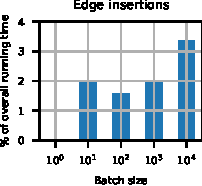
\includegraphics[width=.9\textwidth]{sources/plots/dyn-mwm/breakdown-road-insertion.pdf}
\end{subfigure}\hfill
\begin{subfigure}[b]{.5\textwidth}
\centering
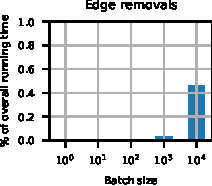
\includegraphics[width=.9\textwidth]{sources/plots/dyn-mwm/breakdown-road-removal.pdf}
\end{subfigure}
\caption{Road networks}
\end{subfigure}\hfill
\begin{subfigure}[b]{.5\textwidth}
\begin{subfigure}[t]{\textwidth}
\centering

\includegraphics{sources/plots/dyn-mwm/legend-cplx.pdf}
\end{subfigure}

\begin{subfigure}[b]{.5\textwidth}
\centering
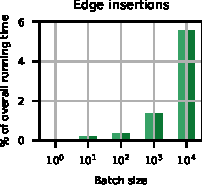
\includegraphics[width=.9\textwidth]{sources/plots/dyn-mwm/breakdown-cplx-insertion.pdf}
\end{subfigure}\hfill
\begin{subfigure}[b]{.5\textwidth}
\centering
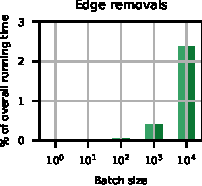
\includegraphics[width=.9\textwidth]{sources/plots/dyn-mwm/breakdown-cplx-removal.pdf}
\end{subfigure}
\caption{Complex networks}
\end{subfigure}
\caption{Percentage of time spent by the static \suitor algorithm for
the preprocessing step (\ie sorting the adjacency lists after a batch
of edge updates) \wrt the overall running time of the algorithm.}
\label{fig:dyn-mwm:breakdown}
\end{figure}

